\documentclass{speauth} 

\usepackage{graphicx}
\usepackage{utils}
\usepackage{requirements}
\usepackage{epsfig}
% The following is enclosed to allow easy detection of differences in
% ascii coding.
% Upper-case    A B C D E F G H I J K L M N O P Q R S T U V W X Y Z
% Lower-case    a b c d e f g h i j k l m n o p q r s t u v w x y z
% Digits        0 1 2 3 4 5 6 7 8 9
% Exclamation   !           Double quote "          Hash (number) #
% Dollar        $           Percent      %          Ampersand     &
% Acute accent  '           Left paren   (          Right paren   )
% Asterisk      *           Plus         +          Comma         ,
% Minus         -           Point        .          Solidus       /
% Colon         :           Semicolon    ;          Less than     <
% Equals        =3D           Greater than >          Question mark ?
% At            @           Left bracket [          Backslash     \
% Right bracket ]           Circumflex   ^          Underscore    _
% Grave accent  `           Left brace   {          Vertical bar  |
% Right brace   }           Tilde        ~

\newcommand{\p}[1]{\texttt{#1}}
\newcommand{\spc}{\textvisiblespace}

\runningheads{M.M. Schrage et al}{Editing structured documents: Requirements} 

\begin{document}
\SPE{0}{0}{0}{0}{2005} 


  \title{Editing structured documents\\ Part I: requirements} 
  \longauthor{Martijn M. Schrage, Johan Jeuring, Lambert Meertens, Doaitse Swierstra}
  \address{Institute of Information and Computing Sciences\\ Utrecht University\\
    Utrecht, The Netherlands}     
\begin{abstract} 
  abstract\dots
\end{abstract}


\section{Introduction} \label{chap:introduction}


%{\em *** Version: \today~ ***}


Many software applications involve some form of editing: a user views a data structure and provides edit gestures in order to modify this data structure. Different kinds of documents require different ways of editing, and hence a multitude of editors exists, each having its own specific edit model and user-interface conventions. Moreover,  since application designers have different ideas on what constitutes a pleasant edit model, even editors for the same document type may show significantly different edit behavior. Nevertheless, the core edit behavior, whether performed in a word-processor or a spreadsheet, is largely similar: document fragments may be copied and pasted, and new parts of the document may be constructed by selecting from menus or entering text. 

% Although gradually, the edit model and user interface of editors seems to become more standard,
% still many differences exist

An obvious research question is to abstract from the specific aspects of each editor and construct a generic system that can be instantiated to a specific editor application. Building an editor with such a system would require only a fraction of the amount of engineering required to build an editor from scratch. 
% And easy to customize. 
A generic editor enhances consistency between editors, because all instantiated editors share the same edit model, and, furthermore, it facilitates the integration of editors for different document types.


%easy to maintain and develop (features added to generic editor
% work in all applications)..

%(also say a gen editor makes it possible to build editors you wouldn't even
% think of building by hand?)

Especially in the nineteen-eighties, many research projects on structure editing were started. However, the editors developed were generally perceived as being overly restrictive, and attempts at developing less restrictive systems resulted mainly in text-only editors. Further, regardless of the restrictiveness of the edit model, the applicability of the generic editors was generally limited to source editors for programming languages and simple word-processing applications.
%No generic editor However, no editor gained much popularity . either  applicable or perceived as restrictive.  but not %one has gained widespread acceptance.
In the years following, research interest in structure editing steadily declined, and many of the generic editors that were developed are now used only for educational purposes at the institute of origin.
%Nowadays, the term structure editor even has a rather negative connotation.

In our opinion, the problem with most of these structure editors is that they either focus on editing the document structure, or the presentation (often just text).
%Lambert: (maar welke structuur-editors focussen op de presentatie en niet op de structuur??)
The document-oriented editors may have a powerful presentation mechanism, but poor editing support in the presentation, which results in a restrictive edit model. On the other hand,  purely presentation-oriented editors lack edit operations on the document, and have relatively weak presentation mechanisms.

% ample support? geeft wel dubbele "there is"
With the increasing popularity of the XML format for representing structured documents, the advantages of a powerful generic editor are becoming even more apparent. Many XML document types are being developed, but support for editing documents of these types is still poor. 
There is a choice between using an expensive custom-made editor, or a generic XML editor, but the functionality of the latter does not come close to what a presentation-oriented (WYSIWYG) editor could potentially offer. It is, for instance, not possible to use any of the current XML editors as a convenient editor for a programming language or for mathematical equations.

In this thesis we investigate whether and how the advantages of structure editing and a powerful presentation formalism can be combined with a non-restrictive presentation-oriented edit model. The result of this research is the presentation-oriented structure editor Proxima.
Before we introduce Proxima, we discuss the basic concepts that play a role in editing structured documents. In Section~\ref{sect:introProxima} we introduce the Proxima editor, followed by a summary of the introduced terminology in Section~\ref{sect:terminology} and an overview of the thesis in Section~\ref{sect:overview}.
\bc
In response to this situation, we have developed  the presentation-oriented structure editor Proxima. The editor can be used for a wide range of applications, such as word-processors or source editors, but also equation editing and spreadsheet behavior is possible. The editor has a layered architecture and combines a powerful document presentation mechanism with a non-restrictive edit model. Besides edit operations on the document structure, the editor also allows editing in the presentation.  A platform-independent Haskell prototype has been implemented, and experiments with instantiated editors have yielded promising results.
\ec

\bc para uit advantages of str editors
Despite the advantages mentioned, generic structure editors are not widespread at all. Several structure editors are used in small communities, but most development projects have been terminated, and in the last decade, very few publications on the subject have appeared. The rise of the XML standard has spawned a large number of generic editors, but when regarded as structure editors, XML editors do not show much variation and do not offer many of the possibilities that a structure editor could offer. Hence, their applicability is limited, and using an XML editor to edit a Java program source, for example, is not possible with the current generation of editors.
\ec



%, and provided promising results.

%Not a monolithic system that takes over the entire os. Just an 
%editor for documents.



%								
%								
%								


\bc
Editing is concerned with the creation and maintenance of documents.  
Most documents have some form of structure. 
\ec

\bc uit Xprez
The popularity of the document standard XML has led to an increasing demand for XML editors. The Proxima project is concerned with the design of a generic presentation-oriented XML editor with support for derived values in documents. A presentation is a view on a document, according to a style sheet. In a presentation oriented editor the user only sees a presentation of a document. WYSIWYG editing is possible using a WYSIWYG presentation, whereas the underlying document structure can be viewed and edited with a presentation that shows the actual tags and tree structure of the document. Because Proxima will support derived values, constructs such as chapter numbers and references are not hard-coded in the editor, but can be specified entirely by the user. Also, computations in a document, where one field contains the result of a calculation over several input fields can be modeled with derived values. In order to specify document presentations, a powerful presentation language is required. For this reason, we have developed the declarative XML presentation language {\sc Xprez}.
\ec




%Word documents, HTML, spreadsheet
%
%Vgl sap-centrifuge Oranges bananas peaches
%juicer, blender, ?
%
%1 Juice Tiger. 
%
% only one machine to buy (and develop) to get used to. different extensions different fruits. Easy to mix different juices.
%
%Generic editor, one system one uniform interface. Easy to combine different documents.
%
%Gelaagde architectuur


% Many applications are editing. view document, enter text, copy paste, move parts, navigate. 
% By abstracting over the specifics of the editor, a generic editor could offer a lot of advantages
% Only one editor for a range of documents provides a uniform interface, and makes embedding documents easy.
% moreover XML: lot of specialized documents that require editing. 
% Even though big ones are hard to replace, generic editor can create easily custom editors with advanced functionality

% in the eighties many projects started: Structure editors. Restrictive never popular. Term structure editor is negative.

% Proxima is a generic editor with a number of features that make it possible to apply it to a wide range of applications

% Although the research in this thesis is not specifically tailored for XML, many of the results apply to XML as well, since 
% XML documents are tree-structured documents. 


% identify problems, and propose an architecture with several novel features that .

% ? instead of have formalism for creating fast and safe editors. We want a formalism that allows us to create the editors
% ? we need. Otherwise these have to be built by hand. 

% prototype has been implemented and although still lot of work to do. It already makes it possible to create editors
% in very little time

% maybe borrow from {Why Proxima} section
% also see ch_conclusions


\section{Preliminaries}

\subsection{Structured documents} \label{sect:structdocs}


%\section{Structured documents}
%Basics of XML and DTD's  Schema. CSS. XSL
%XML is EBNF 
%Documents are trees

A {\em structured document} is a collection of logical entities between which a structural relation exists. Examples of structured documents are HTML pages, program sources, word processor documents, etc. 

In this thesis, we restrict ourselves to structured documents that have a tree structure that can be described by an EBNF grammar. Although graphs can be viewed as structured documents as well, algorithms for performing computations over graphs are far more complex than tree algorithms. Furthermore, parsers for graphs are less well understood than parsers for trees, as well as computationally more expensive. 

In cases where we explicitly want to describe the structure of a document fragment, we use monomorphic (i.e.\ parameter free) Haskell~\cite{peytonJones03haskell} data types together with the list type. Example document fragments are represented by Haskell terms. For example, a document representing the let expression  ``$\mathbf{let}~x = 1;~y = 2~\mathbf{in}~x+y$'' can be denoted in Haskell by: 

\begin{small}
$Let~[Decl~(Ident~\text{``x''})~(Int~1),~Decl~(Ident~\text{``y''})~(Int~2)]~(Sum~(Ident~\text{``x''})~(Ident~\text{``y''}))$
\end{small}
%$Product~(Sum~(Int~1)~(Int~2))~(Sum~(Int 3)~(Int~4))$

\subsection{XML}

The eXtensible Markup Language XML~\cite{xml11} is an increasingly popular standard for representing structured documents. The standard is a simplified descendant of SGML~\cite{sgml86} (Standard Generalized Markup Language). An XML document is a sequence of characters that encodes a tree structure. The nodes of the tree are referred to as {\em elements}. The leaves of the tree are text or attributes (name-value pairs describing properties of an element). The structure of the tree  is represented with opening and closing {\em tags}, and if these tags are nested correctly, the XML document is {\em well-formed}.

The let expression example of the previous section can be represented in XML by:

\ttfamily\begin{small}\begin{tabbing}
<Let><Decl><Ident>x</Ident><Int>1</Int></Decl>\\
~~~~~<Decl><Ident>y</Ident><Int>2</Int></Decl>\\
~~~~~<Sum><Ident>x</Ident><Ident>y</Ident></Sum></Let>
\end{tabbing}\end{small}\rmfamily

%\begin{scriptsize}
%\verb|<Product><Sum><Int>1</Int><Int>2</Sum><Sum><Int val=3><Int val=4></Sum></Product>|
%\end{scriptsize}

The type of an XML document can be specified in several formalisms. The {\em Document Type Definition} (DTD) is part of the XML specification, and basically describes an EBNF grammar over XML elements. A much more expressive formalism is XML Schema~\cite{xmlSchema1}, which itself is a sublanguage of XML. Compared to the DTD formalism, the advantages of using a Schema definition include more control over textual content, as well as a form of inheritance. If an XML document conforms to a certain DTD or Schema, it is called {\em valid}. A third standard, which is not as common as DTDs or Schemas, is the Relax NG standard~\cite{relaxNG01}. Relax NG is a combination of Relax~\cite{relax01} and TREX~\cite{trex01}, and is based on regular expressions. 


%XML is not a meta language.
%Although XML is often referred to as a meta-language, this is not a very accurate term. Indeed, the DTD part of an XML document may %define a language, However, In general, an XML document does not define a language, but is an element of a language. It is only the DTD %description that defines a language. Hence, it would be more appropriate to refer to XML as a super-language.

The number of standards for sublanguages of XML, also referred to as dialects, is rapidly growing. Besides the already mentioned XML Schema, we provide a few more examples.

The Mathematical Markup Language MathML~\cite{mathml20} is a standard for describing mathematical equations and expressions.  \bc Expressions in MathML can be encoded based on  meaning, as well as on presentation. Hence, $1+2$ can be represented either as a sum  element that has two integer child elements, or as a sequence of three elements: two integers with a plus operator in the middle.  \ec Technical documentation can be represented with the DocBook~\cite{walsh02docbook} standard, which exists for XML as well as for SGML. The standard can also be used for papers and books. Finally, we mention the XHTML~\cite{xhtml11} standard, which is an XML encoding of HTML. Although similar, an HTML document is not necessarily an XML document, since HTML is a dialect of SGML rather than XML.


%\note{mention how this thesis relates to XML?}
%** how this thesis applies to XML
%\fromHere

%\verb|<P>Some text with <b>bold</b> and <i>italic</i> words|
%$Para [Text "Some text with", Bold (Text )]$

%Difference between XML and Trees?
%%Difference XML is markup. CFG is tree, everything is part of tree. Markup is more document with tags. leads to differences. 
%things like expressions are awkward to model in XML. On the other hand, mixed... text with bold and bla tags are harder to describe in a %cfg, ...

\subsection{Editing}
\label{sect:editing}


%what is an editor
While the term {\em editor} is usually only associated with plain-text editors such as Emacs~\cite{stallman81emacs} or the ubiquitous Microsoft Notepad, we will use the term in a much broader sense. We regard as an editor any application that presents a visual representation of an internal data structure to a user and allows the user to modify this structure. The internal data structure is referred to as the {\em document} and the visual representation is the {\em presentation}. 

%boundaries of editor concept
Obviously, word processors, image editors, and text editors are editors in this view, but there are also some less obvious examples. Take, for example, the preferences pane that is part of most window-based applications. The check boxes, selection lists, and text fields can be seen as a presentation of the preferences of the application. Another example of an application that is not usually regarded as an editor is a file browser. (For a description of a file browser as a text editor, see for example Fraser~\cite{fraser80generalizedEditor}.)

\begin{figure}
\begin{small}
\begin{center}
\begin{center}
~\hspace{1.7cm}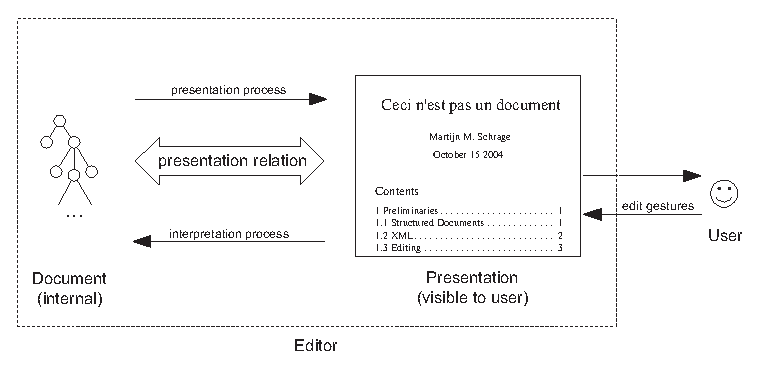
\epsfig{file=pics/eps/editor.eps, width=10cm}
\end{center}\caption{Schematic representation of an editor.}\label{editor} 
\end{center}
\end{small}
\end{figure}

% document and presentation
\vspace*{-1.2ex} Figure~\ref{editor} contains a schematic representation of an editor. The main data structures in the editor (also referred to as {\em levels}) are the internal {\em document} on the left that is not visible to the user and the user-visible {\em presentation} on the right. The document should not be confused with a file, which is a representation of the document that is stored on a file system. Furthermore, we also do not consider an XML source to be a document, but rather a textual presentation of the internal document.

\bc define levels \ec

A {\em presentation}, or {\em view}, is the only thing a user sees of the document. A presentation may be textual, graphical, or a combination of both. We focus on static presentations only. Hence, we do not explicitly consider presentations containing sounds or animations, unless presented statically (e.g.\ as a textual link to a sound or video file). In the presentation, the editor shows the focus of attention, or, for brevity, just {\em focus}, which is a shared name for the selection as well the cursor (which is an empty selection).  Several presentations of a single document may be shown simultaneously by the editor, each having its own focus. Finally, if a presentation closely mirrors the final physical appearance of the document when it is printed, it is referred to as a WYSIWYG presentation (What You See Is What You Get).

% what is presenting
The relation between a document and its presentation is denoted by the term {\em presentation relation}, or {\em presentation mapping}. If, according to the presentation relation, the presentation shown to the user is a presentation of the document, we say that the {\em presentation invariant} holds. Computing the presentation of a document is called the {\em presentation process}, whereas computing a document from a presentation is called the {\em interpretation process}. Together, the two processes implement the presentation relation and maintain the presentation invariant if either side of the relation changes.

% what is valid
A presentation is {\em valid} if there exists a document, which, when presented, yields that presentation. A presentation for which there is no corresponding document is invalid. An invalid presentation may result from an editing the presentation level. Note the difference with the term valid document, which denotes a document that is well typed.

\bc
When the presentation level is a presentation of the document, we refer to it as valid. This should not be confused with valid for XML documents which means type correct.
also in defs
\ec

% what is sheet
The presentation relation for an editor may be (partially) specified in a style sheet, or {\em presentation sheet}. A presentation sheet describes how elements of the document type are to be presented, and is a parameter of the presentation process. By modifying the sheet, a user may influence the appearance of the document without having to modify the editor itself. A presentation sheet can be regarded as a parameter to the interpretation process as well, since the interpretation depends on the presentation specified in the sheet. Examples of style-sheet formalisms are the Cascading Style Sheets (CSS)~\cite{css2} for HTML as well as XML, and the Extensible Stylesheet Language (XSL)~\cite{xsl10} for XML.

%what is the editing process
Generally speaking, editing consists of repeated interactive cycles of presenting and interpreting. The editor shows a presentation of the document together with the current focus to the user. The user then provides the editor with an {\em edit gesture}, such as a key press or a mouse movement, which is interpreted as an update on the document. The document is then re-presented and shown to the user. The process is repeated until the user quits the editor. Chapters~\ref{chap:informalSpec} and~\ref{chap:formalSpec} provide a more formal description of the editing process.

\head{Document-oriented versus presentation-oriented editing}

% doc-oriented vs pres-oriented 
Because edit gestures may be targeted either at the document or the presentation, we distinguish two kinds of editing:  {\em document-oriented} versus {\em presentation-oriented} editing.

% also say document editing/presentation editing?

On the one hand, we have {\em document-oriented editing}, which consists of edit operations (including navigation and selection) that are targeted at the structure of the document rather than at its presentation. Examples are swapping two chapters in a word processor, selecting an entire chapter, or navigating to a next section.

On the other hand, {\em presentation-oriented} editing consists of edit operations on the presentation, which do not necessarily make sense at the document level. If a presentation is textual,  presentation-oriented editing amounts to freely editing the text. As an example, take the mathematical expression  
$(1+2) \times (3+4)$. Deleting the middle part $(1+\framebox{$\,2) \times ($}\,3+4)$ yields $(1+3+4)$ and is a presentation-oriented edit operation that does not directly correspond to a logical operation on the document level. Another example is navigating downwards in a formatted paragraph of a word processor, since the concept of lines in a paragraph only exists at the presentation level. 

Section~\ref{sect:intrProcess} provides a more thorough discussion of both document- and presentation-oriented  editing. Furthermore, the section discusses editing at several other levels, which are introduced at the beginning of Chapter~\ref{chap:proxArch}.
%doc editing is usually also pres editing

\head{Different kinds of editors}

%what is structure editor
The term {\em structure editor} is used to make explicit that an editor has document-oriented editing functionality (also including navigation). We do not make a sharp distinction between plain-text editing and structure editing. Instead, we regard all editing as structure editing, but with a varying level of structure. A text editor can be seen as a structure editor with a very simple structure model: a string or a list of strings. Document-oriented and presentation-oriented editing coincide for a text editor.

%what is generic?
An editor is a {\em generic editor} if it is not specifically built for a single document type but can be used to edit a whole class of document types. A generic editor may be {\em instantiated} to yield an editor for a specific document type. Genericity can be achieved with a single generic editor that edits documents of arbitrary types, but also with an editor generator. An {\em editor generator} is an environment that generates an editor application based on descriptions of the document type and its presentation. Although a generator is not as versatile as a single generic editor, we view both as generic editors. 

%structure editor is not nec. generic
For brevity, we will often adopt the common practice that the term structure editor implies genericity as well. Still, structure editors that are not generic are quite common. A few examples are: equation editors, bookmark editors in web browsers, and file browsers. On the other hand, a generic editor is always a structure editor since it knows about the type of the document.


%??maybe introduce XML Editor here? and forward ref?

%who is the user of a generic editor?
In the context of generic editing, the term {\em user} is ambiguous. A user can either be an editor designer, who instantiates the generic editor for a specific domain, or a user who is editing a document. Unless explicitly stated otherwise, we use the term for the document-editing user.


\bc
When regarded as an editor, more sophisticated input fields that incorporate parsers, may be used. Furthermore, normal undo/redo functionality is possible, instead of the course grained OK/Cancel model, which only allows accepting or ignoring all changes at once.
\ec

\bc
% misschien niet zo'n interessante para
With such a broad view of editors, it is possible to regard every application, and even an entire operating system as an editor. In essence, all a computer user does is give edit gestures with the mouse and the keyboard in response to the presentation on the computer monitor. In reaction to the edit gestures, the internal state of the computer changes, giving rise to a new presentation. 

% en nog een
There is no fundamental problem with this view, but we do not adopt it because a definition that is too broad does not help in finding appropriate abstractions for a generic structure editor. Therefore, we do not explicitly consider all applications to be editors, but adopt the view that many applications contain editors.
\ec


Because it is difficult to give a precise definition of a generic structure editor and because such a definition might be restrictive, we will discuss a number of typical use cases to clarify what we mean by a generic structure editor. Section~\ref{sect:usecases} presents these use cases.





%								
\subsection{Advantages of generic structure editors}

An editor that knows about the structure of the edited document can offer interesting functionality. We list several potential advantages of generic structure editors. The first two advantages stem from the genericity of the editor, whereas the rest are mainly about the structural (document-oriented) abilities.

\begin{description}
\item[Uniform user interface/edit model.] Rather than a separate editor application for each type of document, a single generic editor can be used for a range of document types. Thus, instead of having to cope with several slightly different interfaces, a user only needs to deal with a single uniform interface and edit model.

\item[Integration of documents.] Besides offering editors for different types of documents, a structure editor also facilitates the integration of different types of documents into a single editor instantiation. Thus, it is relatively easy to build an editor for a specific document type, with advanced functionality for the different kinds of edit. Examples are a word-processing editor with spreadsheet functionality, or an editor for slide shows that has syntax coloring and type checking for program code appearing in the slides.

\item[Different Views on the Document.] A structure editor may provide a user with several editable views on the document. The views can show the document in a different order, or with a varying amount of detail. 

\item[Graphical Views.] A view may contain color and fonts in order to clarify document structure, but also use layout alignment, and graphical elements such as lines and boxes.

\item[Derived Information in the Presentation.] The editor can analyze the document during editing and display information computed from the document structure. Examples are the results of static analysis and type checking in source editors, but also chapter numbers or an automatically generated table of contents.

\item[Structural Edit Operations.] Certain edit operations, such as demoting a section with subsections to a subsection with subsubsections in a scientific article, are straightforward to specify at the structural level, but awkward at the presentation level.

\item[Structural Navigation.] Navigating over the document structure instead of its presentation can be very useful. In a source editor, when the focus is on an identifier, a user may easily navigate to its definition in the source. Furthermore, an outline view of the document can be shown in which a user can click to navigate to the corresponding position in the document.

\item[Integration with Other Tools.] A structure editor allows fine control over integration with other tools, such as spell checkers, program-transformation systems, and theorem provers. Furthermore, the editor may show the results coming from these tools at the appropriate position in the presentation, rather than as a list of messages with line numbers.


\end{description}

For document types with a textual presentation, such as program sources or XML documents, some of the advantages can be simulated with a text editor. Lexical analysis can be used on the edited text, and basic support for syntax coloring, auto-completion, and navigation can be provided. However, although simple and efficient, these solutions are  very basic and prone to errors, because, in general, much of the structure of a document cannot be recognized at a purely lexical level.

\bc
sometimes basic structural navigation.  Even though some of the document structure can be recognized at lexical level, in the general case, a full parse is needed. For example, when trying to specify a Haskell function definition as a line in which a '=' character is present, also lines containing strings or comments with '=' characters are identified as function definitions. In some cases the problems can be overcome, but in general this amounts to building a parser in a formalism that is too weak for that purpose. Therefore, we will not consider text editors in this overview of editors.
%*********************************
\ec

% maybe say we  explain why this is the case
% maybe say we will change it? or put that in outline?

% pan article




%								
\subsection{Classes of structure editors} \label{sect:classes}

Three classes of structure editors are distinguished in the literature: {\em syntax-directed}, {\em syntax-recognizing}, and {\em hybrid} editors. Syntax-directed editors mainly support edit operations targeted at the document structure, whereas syntax-recognizing editors support edit operations on the presentation of the document. A hybrid editor combines syntax-directed with syntax-recognizing features, but the term is not used consistently. 
%To avoid confusion, we will refrain from using the term hybrid, except in the brief discussion below.

\head{Syntax-directed editors} 
% mention that structure editing is often source editing.

The first structure editors that were developed are the {\em syntax-directed}, or {\em pure}, structure editors~\cite{reps84synGen,Bahlke86PSG,magnusson90orm}.

Early syntax-directed editors show a textual presentation of the document (usually a program source) but exclusively offer edit operations targeted at the internal document structure, and not at the textual presentation. The original idea behind this was that if structural edit operations are available, a user would not need the textual edit operations anymore. Further, presentation-oriented edit operations would interfere with the user's structural model of the document and introduce errors. Hence they were prohibited altogether. Most editors for XML (see also Section~\ref{sect:xmlEditors}), as well as editors for preferences panes, can be regarded as syntax-directed editors.




\begin{figure}
\begin{small}
\begin{center}
\begin{center}
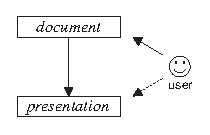
\epsfig{file=pics/eps/SynDirEditor.eps, width=3.5cm}
\end{center}\caption{A syntax-directed editor.}\label{synDirEdit} 
\end{center}
\end{small}
\end{figure}


Figure~\ref{synDirEdit} shows a schematic representation of a syntax-directed editor. The editor works by computing a presentation of the internal document structure, which is shown to the user together with a current focus of attention. The user provides an intended edit operation (edit gesture) on the document structure, from which a document update is computed. After the document is updated, a new presentation is computed, which is shown to the user.

If the editor supports clicking in the presentation to set the focus, the editor also needs to keep track of the origin in the document for each position in the presentation.

In the figure, the line between the user and the presentation is dotted because syntax-directed editors do not support edit operations on the presentation very well. Because the presentation is derived from the document, the editor needs to interpret the intended edit operation on the presentation as an edit operation on the document, which is difficult if the edit operation is not a logical operation on the document level.

A major problem with syntax-directed editors is the restrictiveness of the edit model (e.g.~\cite{vanter94practical,rubinNeal87design}). New structures are easy to create, but not as easy to modify. For example, if a user wishes to change a while statement to an if statement, simply typing over the keyword is typically not supported. 
\finallongpage

Many later syntax-directed editors offer a form of presentation-oriented editing by providing a freely editable textual presentation of (part of) the document, and applying a parser to the edited text. Some publications~\cite{teitelbaum81progSynth, minor90editing} refer to such editors as hybrid, but, as we will explain below, we still regard these editors as syntax-directed editors. 

Unless the two forms of editing are completely integrated, the textual presentation forces a user to work in a different mode of editing, which is referred to as {\em mode switching}. Mode switching does not solve the problem of restrictiveness adequately. Often, a separate window showing a text-only presentation is opened and before the mode can be switched back, the edited text has to be valid. Furthermore, separate modes require a user to be constantly aware of the current mode of the editor. The resulting increased cognitive burden has been shown to be a source of errors~\cite{sellen90modes}.

% mention problems?
\head{Syntax-recognizing editors} 

At the other end of the spectrum are the {\em syntax-recognizing} structure editors~\cite{budinsky85sre, ballance92pan}. A syntax-recognizing editor keeps track of the textual presentation of the document. The user can freely edit the text, and the editor tries to recognize the document structure by means of a parser. Once the text has been (partially) recognized, structural information (e.g.\ syntax-coloring or type information), navigation, and, in some editors, edit operations are available.

\begin{figure}
\begin{small}
\begin{center}
\begin{center}
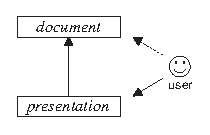
\epsfig{file=pics/eps/SynRecEditor.eps, width=3.5cm}
\end{center}\caption{A syntax-recognizing editor.}\label{synRecEdit} 
\end{center}
\end{small}
\end{figure}

Figure~\ref{synRecEdit} schematically shows a syntax-recognizing editor. The user's edit operations are targeted at the presentation, which can be edited freely. The document is derived by parsing (interpreting) the presentation; hence the reversed direction of the arrow, compared to Figure~\ref{synDirEdit}.

For each element in the document structure, the editor needs to keep track of what parts of the presentation it corresponds to, in order to show structural information in the presentation, as well as support structural navigation. When a document structure has been recognized, the presentation may show additional information using font and color changes, context-sensitive menus, tooltips, etc.
\finallongpage

Similar to the syntax-directed editor, the picture of the syntax-recognizing editor in Figure~\ref{synRecEdit} also contains a dotted arrow. In this case, because the document is derived from the presentation, structural edit operations on the document are difficult to support. A document-oriented edit operation has to be mapped onto an update on the presentation, in such a way that parsing the updated presentation returns the intended updated document. Presentation information that is not stored in the document tree, such as whitespace and comments, has to be related to the document tree in some way, in order to be put in the right place after a structural edit operation.

The main problem with syntax-recognizing editors lies in their limited applicability. Because the presentation needs to contain enough information to derive the document, interesting presentations that only show part of the document are hard to support. Furthermore, graphical presentations, as well as presentations containing computed values and structures, do not fit the model, as these are difficult to parse. As a result, syntax-recognizing editors are mainly limited to text-oriented applications, such as program-source editors.

% mention: good for program editing?
\head{Hybrid editors} 


A {\em hybrid} editor supports structural as well as presentation-oriented edit operations. Figure~\ref{hybridEditor} shows a hybrid editor. Because both levels can be edited, there are no dotted arrows in the figure. However, in order to offer this edit functionality, the editor must realize both the presentation and interpretation mappings. Hence the double arrow between the document and the presentation. 

In some publications (e.g.~\cite{teitelbaum81progSynth, minor90editing}), the term hybrid is used to refer to syntax-directed structure editors that have a limited form of syntax-recognizing functionality. As a consequence, most syntax-directed editors would qualify as hybrid editors, because most editors support some form of text parsing.

In contrast, other publications (e.g.~\cite{ballance92pan, koorn92gse}) advocate that the term hybrid should be reserved for editors that support full textual editing of the document, as well as limited syntax-directed functionality, even if structural modifications on the document are not supported. According to this view, almost all syntax-recognizing editors would classify as hybrid editors, since most of these editors support a form of structural navigation.

Because of the confusion, and because most editors tend to be either primarily syntax-directed or syntax-recognizing, we will often use those terms, instead of the term hybrid.


\section{Proxima} \label{sect:introProxima}

\begin{figure}
\begin{minipage}[b]{.47\textwidth}
    \begin{center}   
~~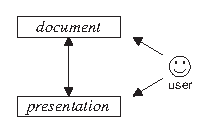
\epsfig{file=pics/eps/HybridEditor.eps, width=3.7cm}
\vspace{56.4pt}
      \caption{A hybrid editor.}\label{hybridEditor} 
    \end{center}
  \end{minipage}
\hfill
\begin{minipage}[b]{.47\textwidth}
    \begin{center}  
\hspace*{0.5cm}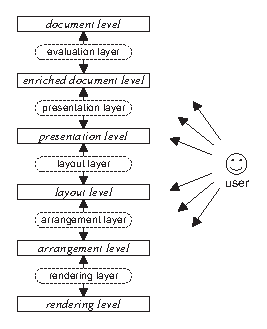
\epsfig{file=pics/eps/ProximaEditorLayers.eps, width=4.8cm}
%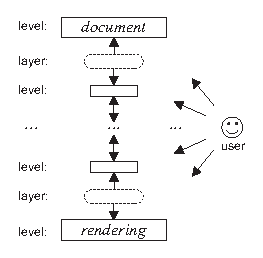
\epsfig{file=pics/eps/ProximaEditor.eps, width=4.7cm}
      \caption{Proxima.}\label{proximaEditor} 
    \end{center}
  \end{minipage}
\end{figure}


The subject of this thesis is the design of the presentation-oriented structure editor Proxima. Proxima is suitable for a wide range of applications, including word-processors and source editors, but also mathematical-equation editors and spreadsheets. An important aspect of Proxima is that the editor fully supports presentation-oriented as well as document-oriented editing. Thus, the editor classifies as a hybrid structure editor.

The implementation of the bidirectional mappings between the document and the presentation is facilitated by a layered architecture. The computation of the presentation is broken up in several stages, and each intermediate value in this computation corresponds to a {\em data level} (or just {\em level}). The interpretation process has the same intermediate values. Between two levels, there is a {\em layer}, which is a component that takes care of mapping values at one level onto values at another level, and thus implements a single stage of the presentation and interpretation processes. 

\bc
Figure~\ref{proximaEditor} sketches the levels and layers of Proxima. Because the name {\em presentation} is reserved for one of the intermediate levels, the lowest level is referred to, more appropriately, as the {\em rendering} level. The figure shows multiple edit arrows coming from the user, because edit operations may be targeted at intermediate stages as well. A more detailed discussion of the levels and layers is provided in Chapter~\ref{chap:proxArch}. 
\note{mention sheets?} 
\ec

The first step of the presentation process is that the {\em document} is enriched with computed values and structures, by the evaluator. The resulting {\em enriched document} is mapped onto a logical {\em presentation} in which positions and sizes are specified relatively. The layout layer adds whitespace that is not stored in the document to the presentation, yielding the {\em layout} level. The layout level is mapped onto an {\em arrangement} level, which contains absolute positions and sizes. And finally, the renderer maps the arrangement onto a {\em rendering}, which is made visible to the user. A more detailed discussion of the presentation and interpretation processes is provided in Chapter~\ref{chap:proxArch}.


Figure~\ref{proximaEditor} shows the levels and layers of Proxima. Because the name {\em presentation} is reserved for one of the intermediate levels, the lowest level is referred to, more appropriately, as the {\em rendering} level. The figure shows multiple edit arrows coming from the user, because edit operations may be targeted at intermediate levels as well.

% by breaking up the interpretation problem
The layered architecture makes it possible to combine presentation-oriented editing with a powerful document-presentation mechanism that includes support for derived values and structures. A platform-independent Haskell prototype of Proxima has been implemented, and experiments with instantiated editors have yielded promising results.

%\begin{figure}
%\begin{small}
%\begin{center}
%\begin{center}
%\begin{small}
%\noindent
%\xymatrix@=0.4cm{
%   \dataa{$Document$}  \ar[dd]   &     \\
%                                            & User  \ar[ld]\ar[lu] \\
% \dataa{$Presentation$} \ar[uu] &   \\
%}
%\xymatrix@=0.4cm{
%   \dataa{$Document (Level_0)$}  \ar[d]   &     \\
%   \dataa{$Level_1$}  \ar[d]\ar[u]   &     \\
%   \dots                                           & User  \ar[ldd]\ar[ld]\ar[lu]\ar[luu] \\
% \dataa{$Level_{n-1}$} \ar[u] \ar[d] &   \\
% \dataa{$Presentation (Level_n)$} \ar[u] &   \\
%}
%\end{small}
%\end{center}\caption{Proxima (draft)}\label{synRecEdit} 
%\end{center}
%\end{small}
%\end{figure}

 
% what about backward mapping, no ES needed? Probably won't know this until some more
% research is done on mappings


\section{Terminology}\label{sect:terminology}

We give a brief summary of the terms that were introduced in the previous sections.

\begin{description}
\item[Editor:] Application for creating and modifying documents. In this thesis, the term also used to refer to structure editors and generic editors (or generic structure editors).
\item[Document:] Internal data structure that represents the information that is edited.
\item[Presentation:] Term for a visible representation of the document (also called a {\em View}), as well as for one of the intermediate levels of the presentation process. 
\item[Presentation mapping/relation:] The relation between the document and its presentation.
\item[Presentation-oriented editing:] Edit operation targeted at the presentation:\\ e.g.\ deleting ``\;$+$\;'' from ``$1+2$'', yielding ``$12$''.
\item[Document-oriented editing/Structure editing:] Edit operation targeted at the document: e.g.\ swapping two sections in an article.
\item[Presentation sheet:] Parameter to the presentation/interpretation process. 
\item[Presentation process:] Process of computing the presentation of a document.
\item[Interpretation process:] Process of computing a document from a presentation.
\item[Level:] Intermediate value of the presentation/interpretation process, including the document and the presentation.
\item[Layer:] Component that realizes the presentation and interpretation mappings between two levels.
\item[Structure editor:] An editor that has knowledge of the structure of the edited document. Usually assumed to be a {\em generic editor} as well.
\item[Generic editor:] A structure editor suitable for editing documents of different types.
\item[Syntax-directed editor:] An editor that primarily supports document-oriented editing.
\item[Syntax-recognizing editor:] An editor that primarily supports presentation-oriented editing.
\item[Valid document:] A well-typed document, mainly used in the context of XML.
\item[Valid presentation:] A presentation that is the result of presenting some document.
\item[Focus:] Shared name for cursor and selection.
\end{description} 

%\section{Why Proxima}
%
%(Will be added when all chapters are more or less finished)

%Why proxima
\bc
complex, but:
new stuff:

-extra state
-also editing on all? levels

Document standard XML getting popular, need editors.

interactive transformations, proof editors, rewrite systems
structural data complex presentations: math
programs with types and structural edit ops: IDEs

Proxima not about changing the world: struct editors, views.  editors have illogical/inconsistent features. Easiest to start all over with new model, however will frustrate users. Better to have a model that allow to express the familiar edit models. and merge them seamlessly.
\ec




\section{Requirements for a structure editor} \label{chap:requirements}

%{\em *** Version: \today~ ***}


\bc

TODO: change wordprocessor screenshot to actual thesis chapter text

Whitespace in use cases
Layout/captions of screenshots

Add Eclipse!





Mention OpenDoc, Views? Not really structure editors.

mention that instead of preventing syntax errors, continuous parsing with in-place error 
info is a good model as well?

incrementality  has been removed from this chapter
Also, we have not paid much attention to incrementality. The layered architecture of Proxima allows incrementality issues to be dealt with by individual layers. 

With current computer speeds, parsers are so fast that incremental parsing has become %less of an issue. We expect that a rather coarse model for incrementality in the %presentation will be sufficient for creating fast editors.
\ec

\bc
Editing is concerned with the creation and maintenance of documents.  
Most documents have some form of structure. 

In this chapter, we give a rather informal definition of editing (editor?**), and look at why no str eds. From a number of use cases, we state a number of requirements that are important in the design of a generic structure editor. Other structure editors are evaluated on these requirements, and . We end with a discussion why no structure editor has yet .  give fun. req. and evaluate related work according to them. End with a discussion why no editor meets all requirements, and how Proxima will.
\ec



\newcommand{\editScrshot}[3]{\fbox{%
\parbox{#1mm}{
\begin{center} #2\\
{\vspace{3mm}\small #3}
\end{center}
}}}
%\newcommand{\thenn}{\hspace{\stretch{1}}$\Rightarrow$\hspace{\stretch{1}}}
\newcommand{\thenn}{\hspace{1mm}$\Rightarrow$\hspace{1mm}}


\newcommand{\editStepScrshot}[4]{%
\begin{center}
\hspace{\stretch{1}}\fbox{
\begin{tabular}[c]{@{}c@{}} \\ [-3mm]
#1 \\ [1mm]
\end{tabular}
}
\thenn
\fbox{
\begin{tabular}[c]{@{}c@{}} \\ [-3mm]
#2 \\ [1mm]
\end{tabular}
} \hspace*{\stretch{1}} \nopagebreak[4] \\ [3mm]
\nopagebreak[4] \hspace*{#3}{#4}\\
\end{center}}

\newcommand{\editStepScrshotChk}[4]{% for figuring out alignment of caption under the arrow
\editStepScrshot{#1}{#2}{#3}{#4}
\begin{center}
$\Rightarrow$\\
{#4}
\end{center}
}

\newcommand{\editStepScrshotSz}[5]{%
\editStepScrshot{\parbox{#1}{#2}}{\parbox{#1}{#3}}{#4}{#5}
}

Many software applications involve some form of editing: a user views a data structure and provides edit gestures in order to modify this data structure. Different kinds of documents require different ways of editing, and hence a multitude of editors exists, each having its own specific edit model and user-interface conventions. Moreover, since application designers have different ideas on what constitutes a pleasant edit model, even editors for the same document type may show significantly different edit behavior. Nevertheless, the core edit behavior, whether performed in a word-processor or a spreadsheet, is largely similar: document fragments may be copied and pasted, and new parts of the document may be constructed by selecting from menus or entering text. 

An obvious research question is to abstract from the specific aspects of each editor and construct a generic system that can be instantiated to a specific editor application. Building an editor with such a system would require only a fraction of the amount of engineering required to build an editor from scratch. A generic editor enhances consistency between editors, because all instantiated editors share the same edit model, and, furthermore, it facilitates the integration of editors for different document types. 

Especially in the nineteen-eighties, many research projects on structure editing were started. However, the editors developed were generally perceived as being overly restrictive, and attempts at developing less restrictive systems resulted mainly in text-only editors. Further, regardless of the restrictiveness of the edit model, the applicability of the generic editors was generally limited to source editors for programming languages and simple word-processing applications. In the years following, research interest in structure editing steadily declined, and many of the generic editors that were developed are now used only for educational purposes at the institute of origin. 

In our opinion, the problem with most of these structure editors is that they either focus on editing the document structure, or the presentation (often just text). The document-oriented editors may have a powerful presentation mechanism, but poor editing support in the presentation, which results in a restrictive edit model. On the other hand, purely presentation-oriented editors lack edit operations on the document, and have relatively weak presentation mechanisms. 
 
With the increasing popularity of the XML format for representing structured documents, the advantages of a powerful generic editor are becoming even more apparent. Many XML document types are being developed, but support for editing documents of these types is still poor. There is a choice between using an expensive custom-made editor, or a generic XML editor, but the functionality of the latter does not come close to what a presentation-oriented (WYSIWYG) editor could potentially offer. It is, for instance, not possible to use any of the current XML editors as a convenient editor for a programming language or for mathematical equations. 

In this paper we investigate requirements for structure editors. We present five use cases in detail. The use cases serve to illustrate the term generic editor, and to formulate requirements for structure editors. 

Section~\ref{sect:usecases} presents the use cases. From these use cases we formulate a set of functional requirements for a flexible non-restrictive structure editor in Section~\ref{sect:reqs}. Existing editors are evaluated according to these requirements in sections~\ref{sect:editorOverview} and~\ref{sect:discussion}, showing why none of these editors can handle all use cases. Finally, in Section~\ref{sect:proxEditor} we discuss how Proxima, a generic structure editor developed at Utrecht University, meets the requirements and thus will be able to implement all of the use cases.

\section{Use cases} \label{sect:usecases}


Some of the five example editors, presented in this section, are well-known applications of structure editors, but a few more exotic applications have been included as well. None of the current generic structure editors can handle all five use cases. It is important to note that although the use cases are discussed as separate applications, aspects of them can be combined in a single editor instance.
The discussion of the edit behavior is illustrated with fictitious screenshots. Actual screenshots of the Proxima prototype can be found in Chapter~\ref{chap:prototype}.



%								
\subsection{A source editor for Haskell}  \label{sect:sourceeditor} 

As an example of a program-source editor, we take an editor for the functional programming language Haskell~\cite{peytonJones03haskell}. The editor supports an extended form of syntax highlighting, in-place display of syntactic and semantic errors, and a range of language-specific edit operations. 

There exists evidence showing that syntax highlighting makes programs more readable~\cite{baecker88readability,omanCook90typography}. Our editor supports highlighting at a semantic rather than syntactic level. Hence, unlike most text editors, the editor can use different display styles for language constructs that are hard to recognize purely syntactically. The type declarations in the next screenshot are an example of such a construct. Although syntactically identical, identifiers in type expressions are colored differently from identifiers in ordinary expressions.

%mention module handling etc.?
 
%$\langle$Haskell listing with syntax coloring and type information$\rangle$
%(also type decls) type info in layered menu? (see text below) 
\begin{center}
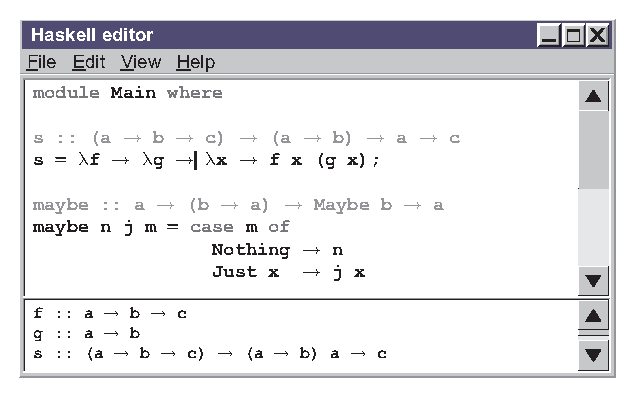
\epsfig{file=pics/eps/HaskellWindow.eps, height=4.5cm}\\ [3mm]
{\sf The Haskell source editor.}
\end{center}

Haskell is a particularly interesting language for a source editor because, due to Haskell's rich type system, information about types is very useful during programming. Haskell programmers often experience that once type errors have been removed, a function is correct. Therefore, an environment that supports in-place display of type errors, as well as easy access to type information of variables in scope, will help rapid program development. 

The upper pane of the editor in the screenshot shows a highlighted source of a simple Haskell module. The bottom pane shows the automatically derived types for identifiers that are in scope at the focused position, including the types of locally declared identifiers. A mouse click on an identifier in the list changes the focus to the definition of that identifier in the source pane. 

%Because many identifiers may be in scope, the menu is layered according to scope level. 

%

\head{Automatic layout/pretty printing}

Some structure editors use an automatic layout scheme while editing program sources. The user then does not need to worry about layout issues, such as the alignment of parameters in functions with multiple clauses. However, for a Haskell editor this situation is not optimal because Haskell programs mainly consist of expressions, which are hard to layout automatically. Therefore, rather than having automatic layout be continuously performed on the entire source, a user may request the editor to automatically lay out a selected part of the program. The specification of the layout of the program is part of a presentation sheet and may be adapted by the user. Of course, if desired, it is also possible to turn on continuous automatic layout.
\vspace{1em}

\newcommand{\editScreenshot}[4]{%
%
\noindent
\begin{center}
\begin{picture}(350,135)(0,0)
\begin{scriptsize}
\put(0,30){ \framebox(160,105){#1}}
\put(180,30){ \framebox(160,105){#2}}
\end{scriptsize}
\put(165,80){ $\Rightarrow$}
\put(0,0) { \makebox(160,30){#3}}
\put(180,0) { \makebox(160,30){#4}}
\end{picture}
\end{center}
}

\newcommand{\editScreenshotTrnsSz}[4]{%
%
\noindent
\begin{center}
\begin{picture}(350,130)(0,0)
\begin{scriptsize}
\put(0,30){ \framebox#1{#2}}
\put(180,30){ \framebox#1{#3}}
\end{scriptsize}
\put(165,80){ $\Rightarrow$}
\put(96,0) { \makebox(150,30){#4}}
\end{picture}
\end{center}
}

\newcommand{\editScreenshotTrns}[3]{%
%
\editScreenshotTrnsSz{(160,105)}{#1}{#2}{#3}
}

\editScreenshotTrns{
\ttfamily 
\begin{tabular}[t]{@{}l@{}}
\begin{tabular}[t]{@{}l@{}}
tails~::~[a]~->~[[a]]\\
tails~[]~=~[[]]\\
tails~xxs@(\_:xs)~=~xxs:tails~xs\\
\end{tabular}
\\
\begin{tabular}[t]{|@{}l@{}|}
\hline
prefix~::~(Eq~a)~=>~[a]~->~[a]~->~Bool\\
prefix~[]~\_~=~True\\
prefix~\_~~[]~=~~False\\
prefix~(x:xs)~(y:ys)~=~if~x~==~y~then\\
~~~~~~~~~~~~~prefix~xs~ys~else~False\\
\hline
\end{tabular}\\
\\
\begin{tabular}[t]{@{}l@{}}
suffix~::~(Eq~a)~=>~[a]~->~[a]~->~Bool\\
suffix~x~y~=~reverse~x~`prefix`~~reverse~y\\
\\
\end{tabular}
\end{tabular}
\rmfamily
}
{
\ttfamily 
\begin{scriptsize}
\begin{tabular}[t]{@{}l@{}}
\begin{tabular}[t]{@{}l@{}}
tails~::~[a]~->~[[a]]\\
tails~[]~=~[[]]\\
tails~xxs@(\_:xs)~=~xxs:tails~xs\\
\end{tabular}
\\
\begin{tabular}[t]{|@{}l@{}|}
\hline
prefix~::~(Eq~a)~=>~[a]~->~[a]~->~Bool\\
prefix~[]~~~~~\_~~~~~~=~True\\
prefix~\_~~~~~~[]~~~~~=~False\\
prefix~(x:xs)~(y:ys)~=~if~x~==~y\\
~~~~~~~~~~~~~~~~~~~~~~~then~prefix~xs~ys\\
~~~~~~~~~~~~~~~~~~~~~~~else~False\\
\hline
\end{tabular}\\
\\
\begin{tabular}[t]{@{}l@{}}
suffix~::~(Eq~a)~=>~[a]~->~[a]~->~Bool\\
suffix~x~y~=~reverse~x~`prefix`~~reverse~y\\
\end{tabular}
\end{tabular}
\end{scriptsize}
\rmfamily
}{\small apply layout}

The screenshot shows the automatic-layout operation applied to the selected function {\tt prefix}. The formatted function on the right-hand side is still freely editable, including its whitespace.
% comment handling?

\head{Structural edit operations}

Because a program construct is represented by a contiguous area in the presentation, moving a program construct can usually be done in a straightforward way by moving its presentation. However, this is not always the case. Take, for example, the expression:

\verb|let x=1; y=2 in x+y|

The expression consists of a list of declarations that are separated by semicolons and whitespace. Contrary to, for example, the language Java, the semicolon in Haskell acts as a separator, and not as a terminator. Unlike a terminator, which can be regarded as part of the presentation of a declaration, a separator belongs to the presentation of the list of declarations. As a result, semicolons may cause problems when declarations are moved.

Consider moving the first declaration \verb|x = 1| to the end of the let expression. When the declaration is cut, the semicolon behind it must be deleted, and when the declaration is pasted, a semicolon with appropriate whitespace must be added. Similar issues apply to all list structures that are presented using separators, such as Haskell lists \verb|[1, 2, 3]|, tuples \verb|(1,2,3)|, or monadic \verb|do| expressions: \verb|do {a <- getChar ; putStr [a]}|.

\newcommand{\focus}{\vrule height2ex width0.5pt depth0.8ex}

If the structure of the edited list is taken into account, cut-and-paste on lists with separators can be handled elegantly. When the first declaration is selected, the editor recognizes it as an element of the let expression's declaration list, and when it is cut, the semicolon next to it disappears:

\begin{center}
\hspace{\stretch{1}}
\fbox{
\begin{scriptsize} \begin{tabular}[c]{@{}c@{}} \\ [-2mm]
let \framebox{x=1\strut}; y=2 in x+y    \\ [1mm]
\end{tabular}\end{scriptsize}
}
\thenn
\fbox{
\begin{scriptsize} \begin{tabular}[c]{@{}c@{}} \\ [-2mm]
let \focus$\!$ y=2 in \underline{x}+y    \\ [1mm]
\end{tabular}\end{scriptsize}
}
\thenn
\fbox{
\begin{scriptsize} \begin{tabular}[c]{@{}c@{}} \\ [-2mm]
let y=2\focus~in x+y    \\ [1mm]
\end{tabular}\end{scriptsize}
}
\thenn
\fbox{
\begin{scriptsize} \begin{tabular}[c]{@{}c@{}} \\ [-2mm]
let y=2; \framebox{x=1\strut} in x+y    \\ [1mm]
\end{tabular}\end{scriptsize}
}
\hspace{\stretch{1}}\nopagebreak[4]\\ [2mm]
\begin{small}
\parbox{125mm}{
{\small \hspace*{0.13cm}\hspace*{3.47cm} cut \hspace{1.3cm} move focus  \hspace{1.20cm} paste}}
\end{small}\end{center}

%\editScreenshot{let y=2 in \underline{x}+y}{let y=2; \framebox{x=1\strut} in x+y}{after cut}{after paste}


When the declaration is pasted, a semicolon is automatically placed in front of it. The whitespace from the semicolon is copied from the whitespace of the other semicolons in the presentation (or may come from a pretty-printing algorithm). If the list has an irregular layout (e.g.\ \verb|[1,  2,    3, 4]|), the layout after the paste operation may not be what is expected. However, since list structures are usually layed out in a regular way, this need not be a problem.

If an edit operation can be performed both structurally as well as presentation-oriented, as is the case here, the editor gives preference to the structural edit operation. In order to perform the cut and paste operations from the example on the presentation (and thus leave the semicolon untouched), a modifier key may be pressed.


\head{Rename within scope}

A second example of an edit operation that takes the document structure into account is a rename operation on an identifier. In a regular text editor, occurrences of the identifier name need to be changed using search and replace. However, automatic search and replace does not always lead to the desired result because the identifier may be redeclared in inner scopes, or the identifier name may appear in a string.

\editStepScrshot{\begin{scriptsize} f \framebox{a\strut} b = a + let a = 10 in a \end{scriptsize}}
{\begin{scriptsize} f \framebox{x\strut} b = x + let a = 10 in a \end{scriptsize}}
{0em}{\small rename variable}

% a function is a better example
The rename operation takes account of the scoping rules of Haskell, and only changes the appearances that lie in scope of the updated identifier. If the new name is captured by an inner declaration, or if it shadows an identifier that is already declared, a warning is issued.

The rename operation is an example of a {\em refactoring} operation: a source-to-source program transformation that leaves  the functionality of the program intact. The designers of the Haskell Refactorer~\cite{reinke03refactoring} identify a number of such transformations.

\head{Hide function definitions/folding}

Function definitions in the source presentation may be collapsed, leaving only one left-hand side and the (possibly inferred) type declaration. This operation is often referred to as folding.
\vspace*{1.4ex}

\editScreenshotTrns{
\begin{tabular}[t]{l}
%{\tt yA (LineA \_ x y x' y' \_ \_)~~~= y}\\
%{\tt yA (PolyA \_ x y w h \_ \_ \_ \_)~= y}\\
%{\tt yA (RowA \_ x y w h \_ \_)~~~~~~= y}\\
{\tt yA (ColA \_ x y w h \_ \_)~~~~~~= y}\\
{\tt yA (OverlayA \_ x y w h \_ \_)~~= y}\\
\\
\begin{tabular}[t]{@{}l@{}l}
{\tt widthA :: Arrangement $\rightarrow$ Int}\\
{\tt widthA (StringA \_ x y w h \_ \_ \_ \_)} &\p{ = w}\\
{\tt widthA (ImageA \_ x y w h \_ \_ \_ \_)} &\p{  = w}\\
{\tt widthA (PolyA \_ x y w h \_ \_ \_ \_)} & \p{ = w}\\
{\tt widthA (RowA \_ x y w h \_ \_)} & \p{ = w}\\
{\tt widthA (ColA \_ x y w h \_ \_)} & \p{ = w}\\
{\tt widthA (OverlayA \_ x y w h \_ \_)} & \p{ = w}\\
\end{tabular}
\\
\\
{\tt heightA :: Arrangement $\rightarrow$ Int}\\
{\tt heightA (StringA \_ x y w h \_ \_ \_ \_)~= h}\\
\end{tabular}
}{
\begin{tabular}[t]{l}
%{\tt yA (LineA \_ x y x' y' \_ \_)~~~= y}\\
%{\tt yA (PolyA \_ x y w h \_ \_ \_ \_)~= y}\\
%{\tt yA (RowA \_ x y w h \_ \_)~~~~~~= y}\\
{\tt yA (ColA \_ x y w h \_ \_)~~~~~~= y}\\
{\tt yA (OverlayA \_ x y w h \_ \_)~~= y}\\
\\
 {\tt widthA :: Arrangement $\rightarrow$ Int}\\
{\tt widthA = \framebox{\rule{0cm}{1.5ex}\dots}}\\
\\
\begin{tabular}[t]{@{}l@{}l}
{\tt heightA :: Arrangement $\rightarrow$ Int}\\
{\tt heightA (StringA \_ x y w h \_ \_ \_ \_)}&\p{ = h}\\
{\tt heightA (ImageA \_ x y w h \_ \_ \_ \_)}&\p{ = h}\\
%{\tt heightA (LineA \_ x y x' y' \_ \_)}&\p{ = y'-y}\\
{\tt heightA (PolyA \_ x y w h \_ \_ \_ \_)}&\p{ = h}\\
{\tt heightA (RowA \_ x y w h \_ \_)}&\p{ = h}\\
{\tt heightA (ColA \_ x y w h \_ \_)}&\p{ = h}\\
{\tt heightA (OverlayA \_ x y w h \_ \_)}&\p{ = h}
\end{tabular}
\end{tabular}
}{\small hide function definition}

The two functions \verb|widthA| and \verb|heightA| have a large number of clauses. Hiding these clauses may improve the readability of the source. After applying the {\em hide function body} edit operation to the function \verb|widthA|,  only one clause remains with a collapsed right-hand side (\hspace{0.5pt}{\tt \framebox{\rule{0cm}{1.5ex}\dots}}\hspace{0.5pt}). The function is expanded again by clicking on the dots. A collapsed function may be renamed, deleted, or structurally moved around in the source. Editing the whitespace around the `\verb|=|' sign would be ambiguous because of the hidden parameters names and the fact that a single collapsed function typically represents several clauses. Hence, editing this whitespace is not allowed.

\head{Requirements} % haskell editor

The source editor generates a number of requirements, an important one being the possibility of freely editing the textual program source, including the layout. At the same time, it must be possible to let the layout be computed automatically as well. Furthermore, a formalism for specifying computations over the document is required for performing static analysis and type checking.

Freely editing the program source is not always regarded a requirement for a structure editor. Purists argue that text editing may introduce syntactic errors, and that it is not necessary for programming (e.g.~\cite{teitelbaum81progSynth,magnusson90orm}). However, no clear consensus has been reached on the subject (e.g.~\cite{abandonText82waters} and reactions \cite{shani83notAbandon,responseToWaters83notkin}, and \cite{vanter94practical}) and nowadays most syntax-directed editors support some form of free text editing. Furthermore, because up to now no pure syntax-directed editor has ever become popular with programmers, we believe that free textual editing is an essential requirement for a program-source editor.

%																
\subsection{A word processor} \label{sect:wordprocessor} 

This section describes a WYSIWYG document editor with a user interface similar to word-processing applications such as Microsoft Word, but with a document model similar to the XML/SGML DocBook standard~\cite{walsh02docbook} and an output quality similar to \TeX~\cite{knuth84tex}. Examples of editors with similar functionality are TeXmacs\cite{texmacs} and Lyx~\cite{lyx}, but neither system is generic.
\vspace*{1.4ex}


\newcommand{\screenshotWin}[2]{%
%
\noindent 
\begin{center}
\begin{picture}(225,165)(0,0)
\begin{scriptsize}
\put(-2,30){ \epsfig{file=pics/eps/WordprocessorWindow.eps, height=4.8cm}}
\put(0,132){ 
\begin{tabular}[t]{p{7cm}}
\hfill{\normalsize Proxima}\hfill~\\
\vspace{0.001cm}
\hfill{\scriptsize Martijn M. Schrage}\hfill~\\
\vspace{0.0005cm}
{\small Contents}\\
\vspace{0.0007cm}
~~~1~~Editing~structured~documents\\
~~~2~~Use cases \\
~~~3~~Functional requirements\\
\vspace{0.2cm}
{\small 1~~Editing~structured~documents}\\
\vspace{0.001cm}
\parbox{6.9cm}{While the term {\em editor} is usually only associated with plain-text editors such as Emacs~\cite{stallman81emacs} or\vline~ the ubiquitous Microsoft Notepad, we will ~~~~~~~~~~~~~~~~~\strut
}\\
\end{tabular}
}
%\put(1,33){ 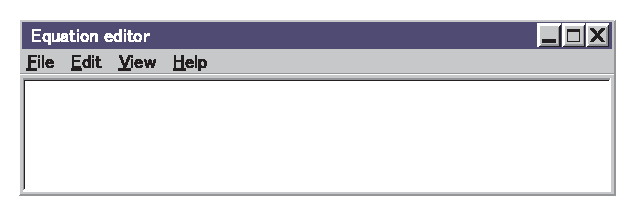
\epsfig{file=pics/eps/EqEdWin.eps, height=102.5pt}}
%\put(1,33){ 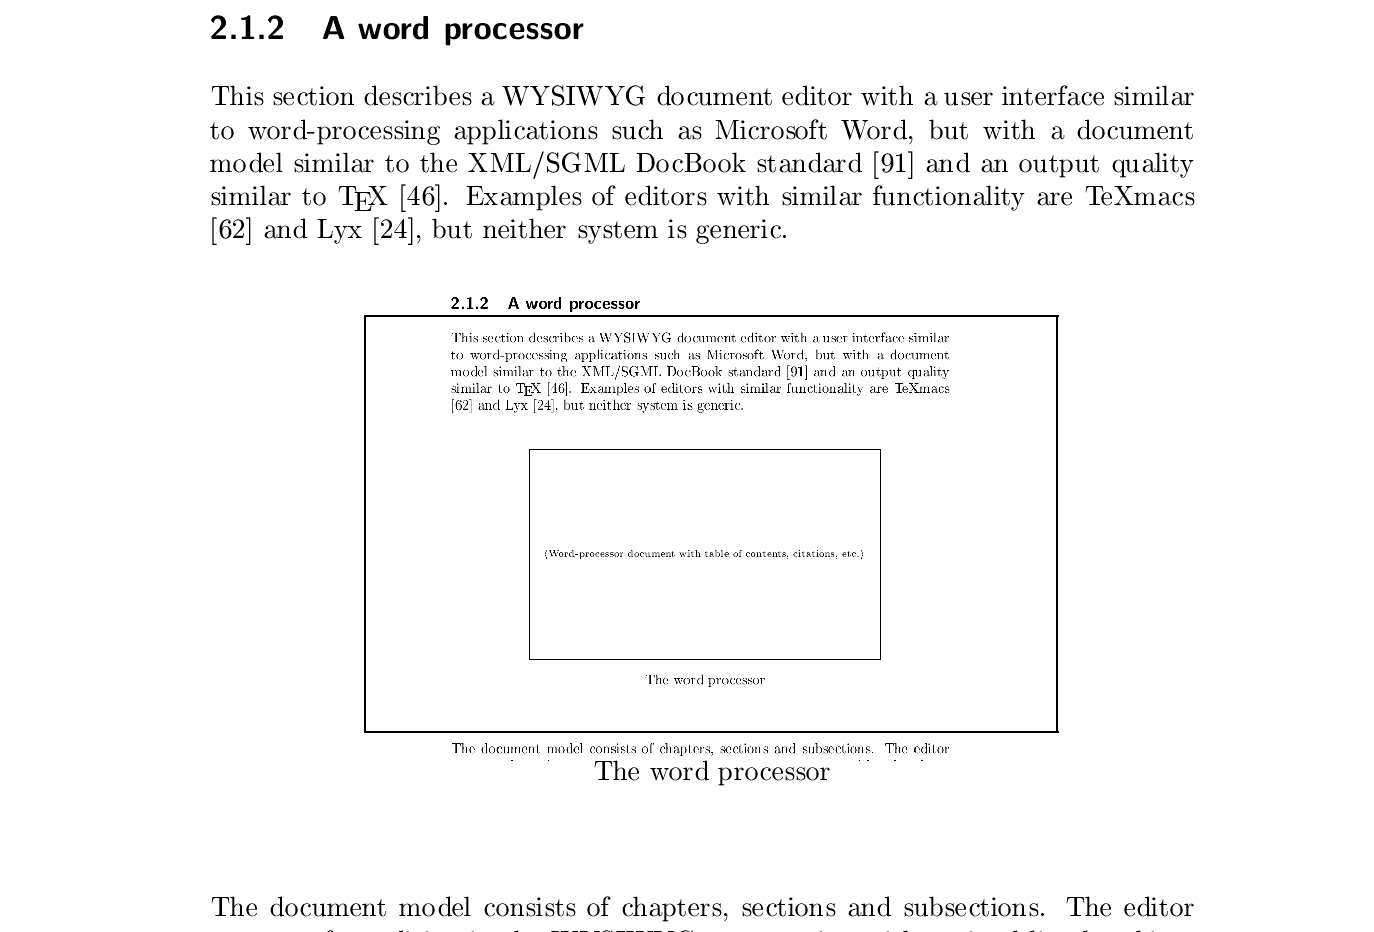
\epsfig{file=pics/screenshots/Wordprocessor.png.eps, height=102.5pt}}
\end{scriptsize}
\put(0,0) { \makebox(190,30){#2}}
\end{picture}
\end{center}
}


\screenshotWin{%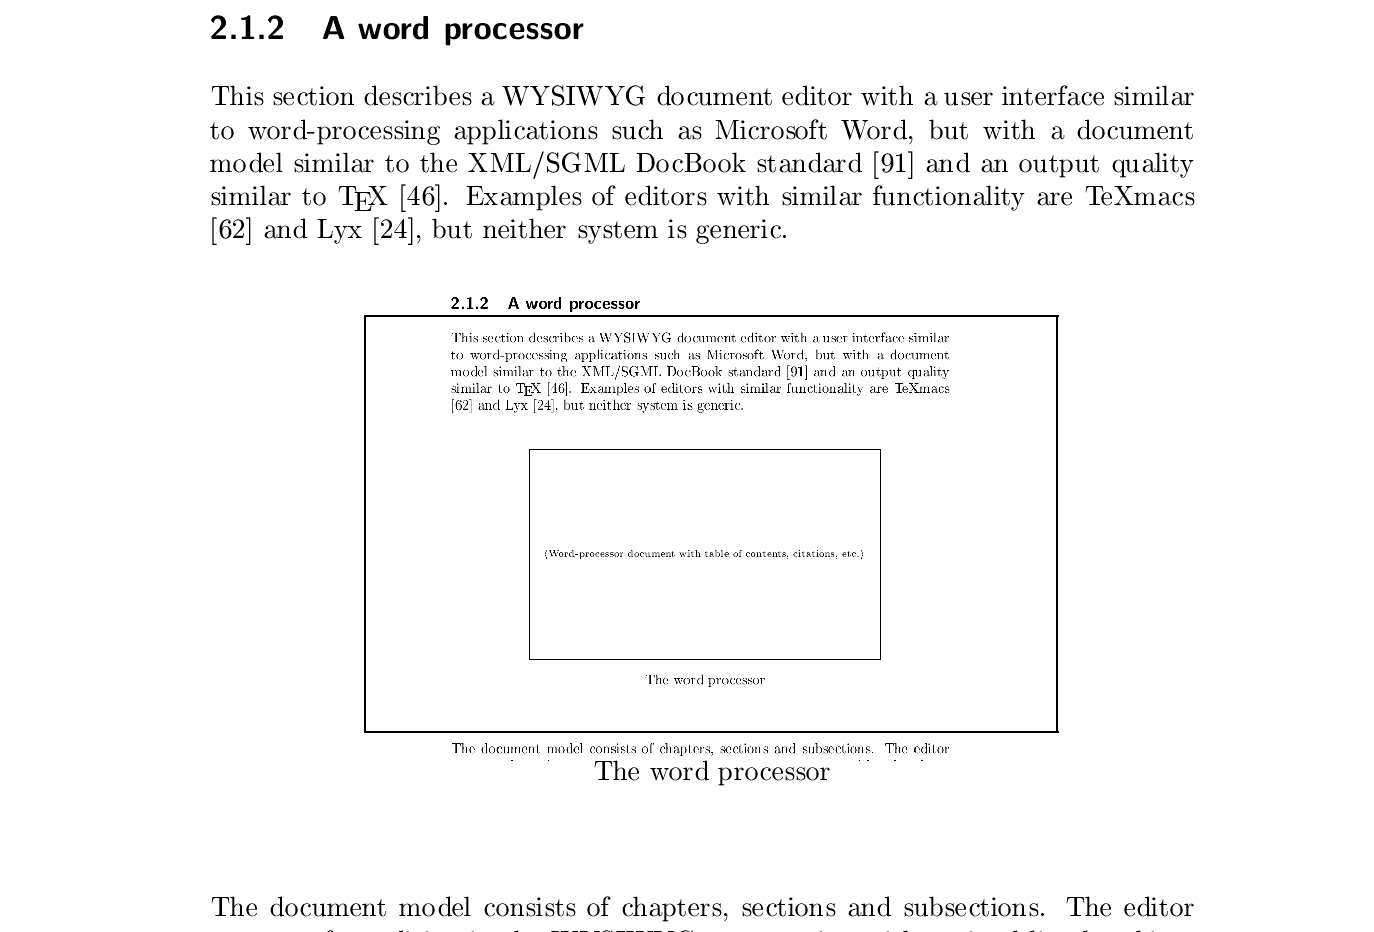
\epsfig{file=pics/Screenshots/Wordprocessor.png.eps, height=6cm}
}{\hspace*{1cm}\normalsize \sf The word processor.}
%$\langle$Word-processor document with table of contents, citations, etc.$\rangle$

The document model consists of chapters, sections and subsections. The editor supports free editing in the WYSIWYG presentation with optimal line breaking, a derived table of contents, and an automatic bibliography. Cross-references, such as citations or references to figures, can be clicked to bring the referred part of the document into focus.

\head{Structural view on the document}

Although Microsoft Word is one of the most popular word-processing tools in the world, an often-heard complaint concerns its confusing document model. Sometimes edit operations are not allowed because of underlying document structure, but it is not obvious why this is the case. Furthermore, the reason why a document fragment looks the way it does is not always clear. The user may have set specific style attributes for a particular fragment, or the style may originate from the document's presentation rules. A more structural view on the document, such as WordPerfect's ``underwater'' screen, can help to clarify the situation, but is not supported by Word. Such a structural view is easily defined in a structure editor:



\editStepScrshotSz{4.5cm}{
\begin{scriptsize}\begin{tabular}{@{}l@{}}
\rmfamily
normal text {\em \vline{\bf \em italic and bold} just italic} normal\\
text again {\bf \em plus a warning}.\\
\end{tabular}
\end{scriptsize}
}{
\begin{scriptsize}\begin{tabular}{@{}l@{}}
normal text $\langle$e$\rangle$\vline$\langle$b$\rangle${\em {\bf \em italic and bold}}$\langle$/b$\rangle$ {\em just}\\
{\em italic}$\langle$/e$\rangle$ normal text again $\langle$Warning$\rangle${\bf \em plus a} \\
{\bf \em warning}$\langle$/Warning$\rangle$.\\
\end{tabular}\end{scriptsize}
}
{0em}{\small switch to structural presentation}


The two screenshots show two presentations of the same document fragment. The left-hand presentation is the regular WYSIWYG presentation, whereas the right-hand one is a more structural presentation that shows the markup tags. The example document also contains a fictitious \verb|<Warning>| element that is presented in a bold and italic style. Only in the structural presentation can the warning be distinguished from text that has been explicitly formatted as bold and italic.

The structural view is also helpful for positioning the focus. In the left-hand presentation it is not clear whether the focus is in the regular text, the italic part, or the part that is both italic and bold. The right-hand presentation, on the other hand, shows the exact position of the focus in the italic part. In order for the structural views to be helpful, the editor supports easy switching between views while preserving the current focus.

\bc
The structural view is also helpful for positioning the focus. For example, in the left-hand presentation, the start of the first piece of italic text just before the bold part coincides with the start of the bold part; therefore inserting text that is italic but not bold is rather tricky. In the right-hand presentation the positions do not coincide and text that is only italic as well as text that is italic and bold can be inserted without a problem. In order for the structural views to be helpful, the editor supports easy switching between views while preserving the current focus.
\ec

%Handles to invisible stuff, attributes?

\head{Structural edit operations}

Edit operations that rearrange the document structure, such as promoting a subsection to section, are awkward to perform on a textually represented document, such as a \TeX\ source. All tags or \TeX\ commands that specify the subsection and its descendants need to be changed. This is a rather specific search/replace operation on only part of the document source, which is a hassle to automate.

A structure editor may be of some help here, because the structural similarities between sections and subsections are known to the editor and can be used to define edit operations for restructuring the document.



\editStepScrshot{
\begin{scriptsize}
\begin{tabular}[t]{@{}l@{}}
\\ [-1.5em] 
{\large Contents}\\ [0.5em]
~~~~1~~Editing~structured~documents\\
~~~~~~1.1~~Classes of structure editors\\
~~~~~~1.2~~Advantages of structure editors\\
~~~~~\,\fbox{1.3~~Use cases}\\
~~~~~~~~1.3.1~~A source editor for Haskell\\
~~~~2~~Functional requirements
\end{tabular}\end{scriptsize}
}{ 
\begin{scriptsize}
\begin{tabular}[t]{@{}l@{}}
\\ [-1.5em] 
{\large Contents}\\ [0.5em]
~~~~1~~Editing~structured~documents\\
~~~~~~1.1~~Classes of structure editors\\
~~~~~~1.2~~Advantages of structure editors\\
~~~\,\fbox{2~~Use cases}\\
~~~~~~2.1~~A source editor for Haskell\\
~~~~3~~Functional requirements
\end{tabular}\end{scriptsize}
}
{0em}{\small change to section}
 
The screenshot shows the effect of the structural edit operation ``change to section''. If the containing section (``Editing structured documents'') had had any subsections following the promoted subsection, these could have become subsections of the new ``Use cases'' section. However, different behavior for such sections may be specified by the user in a preferences window for the edit operation.

An operation that changes the level of a section or subsection is rather complex because it involves splitting and changing elements. Moreover, there are special cases to consider. For example, if a subsubsection is the deepest possible structural level, a warning needs to be issued when a section containing a subsubsection is demoted to subsection. Therefore, such an operation needs to be specified explicitly by the editor designer or user. Other document operations, however, such as splitting and joining elements of a list, may be derived automatically.
% show transf. spec. language?

% link to outline ed, and support moving of structures?

\head{Editing a section title in the table of contents}

The word processor has support for the specification of a generated table of contents. From an entry in the table, a user can jump to the corresponding position in the document presentation. The presentation of the table of contents itself can be customized to match the style of the rest of the presentation. When the document is edited, the table of contents is updated accordingly. Moreover, editing an entry in the table of contents causes an update to the title of the corresponding chapter or section.

\newcommand{\editScreenshotTrnsFrSmall}[3]{%
%
\noindent
\begin{center}
\begin{picture}(350,100)(0,0)
\begin{scriptsize}
\put(5,30){ \makebox(160,75){#1}}
\put(5,30){ 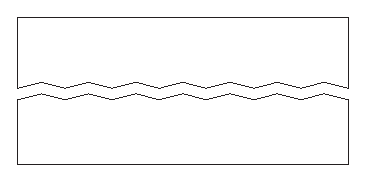
\epsfig{file=pics/eps/frameSmall.eps, height=70pt} }
\put(180,30){ \makebox(160,75){#2}}
\put(180,30){ 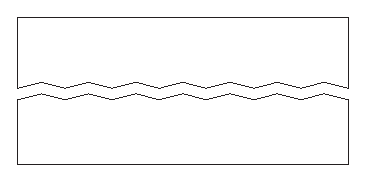
\epsfig{file=pics/eps/frameSmall.eps, height=70pt} }
\end{scriptsize}
\put(165,60){ $\Rightarrow$}
\put(96,0) { \makebox(150,30){#3}}
\end{picture}
\end{center}
}


\editScreenshotTrnsFrSmall{
\begin{tiny}
\begin{tabular}[t]{p{5.2cm}}
\\ [3ex]
{\small Contents}\\
\vspace{0.001cm}
~~~1~~Editing~structured~documents\\
~~~2~~\framebox{$\!$U$\!$}se cases\\
~~~3~~Functional requirements\\
\vspace{0.3cm}
{\small 2~~Use cases}\\
\vspace{0.001cm}
\parbox{5.2cm}{In this section, we present five use cases of possible applications for a generic structure editor. The use cases will shed more light on the defini- ~~~~~~~~~~~~~~~~~\strut
}
\end{tabular}
\end{tiny}
}{
\begin{tiny}
\begin{tabular}[t]{p{5.2cm}}
\\ [3ex]
{\small Contents}\\
\vspace{0.001cm}
~~~1~~Editing~structured~documents\\
~~~2~~The u\vline se cases\\
~~~3~~Functional requirements\\
\vspace{0.3cm}
{\small 2~~The use cases}\\
\vspace{0.001cm}
\parbox{5.2cm}{In this section, we present five use cases of possible applications for a generic structure editor. The use cases will shed more light on the defini- ~~~~~~~~~~~~~~~~~\strut
}
\end{tabular}
\end{tiny}
}{\small enter ``\p{The\spc u}''}
% In final picture maybe use Lambert's idea instead of dots? (3 different blocks, each with zigzag ends)

The screenshot shows a document with a table of contents. The second entry in the table of contents is edited by entering the text ``The u'' over the selected letter `U' at the beginning of the title. The result is that the title in the table of contents as well as the title in the section is updated.

\head{Moving a section in the table of contents}

Besides textual edit operations, it is also possible to perform structural edit operations on derived structures. The screenshot shows a move operation on a section title in the table of contents, which has the result that the corresponding section is moved in the document.


\newcommand{\editScreenshotTrnsFr}[3]{%
%
\begin{center}
\begin{picture}(340,135)(0,0)
\begin{scriptsize}
\put(2,30){ \makebox(160,105){#1}}
\put(2,30){ 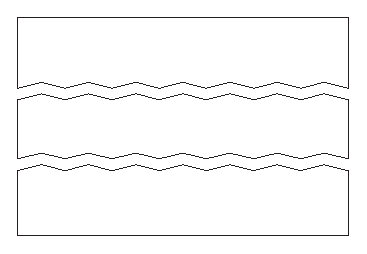
\epsfig{file=pics/eps/frame.eps, height=105pt} }
\put(180,30){ \makebox(160,105){#2}}
\put(180,30){ 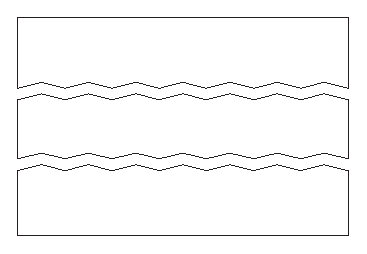
\epsfig{file=pics/eps/frame.eps, height=105pt} }
\end{scriptsize}
\put(165,80){ $\Rightarrow$}
\put(96,0) { \makebox(150,30){#3}}
\end{picture}
\end{center}
}

\editScreenshotTrnsFr{
\begin{tiny}
\begin{tabular}[t]{p{5.2cm}}
\\[0mm]
{\small Contents}\\
\vspace{0.001cm}
~~$\!\,$\framebox{1~~Editing~structured~documents}\\
~~~2~~Use cases \\
~~~3~~Functional requirements\\
\vspace{0.2cm}
{\small 1~~Editing~structured~documents}\\
\vspace{0.001cm}
\parbox{5.2cm}{
While the term {\em editor} is usually only associated with plain-text editors such as Emacs~\cite{stallman81emacs} or the ubiquitous Microsoft Notepad, we will use the 
 ~~~~~~~~~~~~~~~~~\strut
}\\
\vspace{0.07cm}
{\small 2~~Use cases}\\
\vspace{0.001cm}
\parbox{5.2cm}{In this section, we present five use cases of possible applications for a generic structure editor. The use cases will shed more light on the defini- ~~~~~~~~~~~~~~~~~\strut 
}
\end{tabular}
\end{tiny}
}{
\begin{tiny}
\begin{tabular}[t]{p{5.2cm}}
\\[0mm]
{\small Contents}\\
\vspace*{0.034cm}
~~~ 1~~Use cases\\
~~~$\!\,$\framebox{2~~Editing~structured~documents}\\
~~~ 3~~Functional requirements\\
\vspace{0.2cm}
{\small 1~~Use cases}\\
\vspace{0.001cm}
\parbox{5.2cm}{
In this section, we present five use cases of possible applications for a generic structure editor. The use cases will shed more light on the defini- ~~~~~~~~~~~~~~~~~\strut 
}\\
\vspace{0.07cm}
{\small 2~~Editing~structured~documents}\\
\vspace{0.001cm}
\parbox{5.2cm}{
While the term {\em editor} is usually only associated with plain-text editors such as Emacs~\cite{stallman81emacs} or the ubiquitous Microsoft Notepad, we will use the 
 ~~~~~~~~~~~~~~~~~\strut
}
\end{tabular}
\end{tiny}
}{\small move section entry}
%{after drop}

The section entry for the ``Editing structured documents'' section is selected and dragged to its new location, just below the entry for the ``Use cases'' section. The result is an edit operation on the document structure that puts the first section after the second section. The section numbers switch because they are generated automatically. Whenever an edit operation on a derived structure is performed, the user may be signaled that the operation affects more than just the visible selection.

Although structure-changing operations on derived structures may not always make sense, it is important that they can be specified for the cases in which they do.

\head{Requirements} % word processor

Compared to the source editor, the word processor requires a more powerful presentation formalism. Besides text in different fonts, sizes, and colors, the presentation also contains images and basic graphical elements. Furthermore, support for optimal line and page breaking is needed for formatting paragraphs and pages. 

Finally, in order to handle edit operations on the table of contents, the editor must support editing not only on presentation and document level, but also on the level of derived structures.


%																
\subsection{Equation editor/MathML}  

Because mathematical formulas have a high degree of structure, a mathematical equation editor is a good candidate for structure editing. Equation editing functionality is typically integrated with a word processor to support in-place editing of equations in a document. An example of an editor for mathematical documents is the MathSpad editor~\cite{verhoeven00mathspad}, which offers word-processing functionality as well. MathSpad also supports a form of genericity, but does not allow the document type to be specified. Furthermore, both the edit model and the presentation have a tendency towards documents of a mathematical nature.


%The TexMacs and Lyx editors mentioned in the previous section support math editing. 

%However, we separate the two examples here because of the different requirements they generate.

%MathSpad has some support for genericity, but it does not allow definition of document type. 

\newcommand{\screenshotWintwo}[2]{%
%
\noindent 
\begin{center}
\begin{picture}(200,90)(0,0)
\begin{scriptsize}
\put(-2,30){ 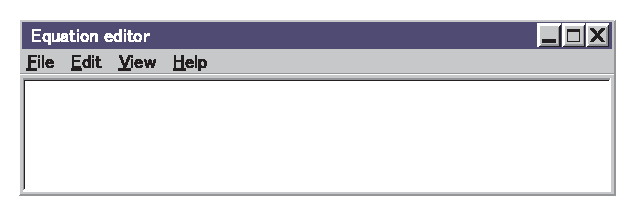
\epsfig{file=pics/eps/EqEdWin.eps, height=60pt}}
\put(5,25){ \makebox(190,50){#1}}
\end{scriptsize}
\put(0,0) { \makebox(190,30){#2}}
\end{picture}
\end{center}
}

\screenshotWintwo{
\parbox{100mm}{\begin{displaymath}
U(\vec{x}_1,\vec{x}_2,t) = 
- \frac{\hbar^2}{R(\vec{x}_1,\vec{x}_2,t)} 
\left( \frac{\nabla^2_1R(\vec{x}_1,\vec{x}_2,t)}{2m_1} +
 \frac{ \nabla^2_{2}\vline}{2m_2} \right)
\end{displaymath}}
% \nabla^2_2R(\vec{x}_1,\vec{x}_2,t)
}{\normalsize \sf The equation editor.}


The screenshot shows a WYSIWYG equation editor with support for mathematical constructs such as fractions, roots, and integrals. A possible document type for  the equation editor is the Mathematical Markup Language MathML~\cite{mathml20}.


Mathematical formulas are suitable for document-oriented edit operations, using menus and buttons for structure entry. Free presentation-oriented editing, on the other hand, is not as clearly defined on a formula as it is on a program source. For example, shrinking the 2 in the number 42 and moving it upwards a bit, could theoretically lead to recognition of the square $4^2$. However, this requires a complicated visual parsing scheme, the exact behavior of which is not clear. Therefore, the editor only allows free editing in the textual parts of a formula that can be parsed unambiguously.

Although such a rather restricted edit model is common even in the current generation of non-generic equation editors, we believe that a more sophisticated and flexible edit model is possible. The Proxima architecture does not prohibit such an edit model, but further research on parsing two-dimensional structures is required before it can be supported.

\head{Drag and drop}

Direct manipulation of parts of the formula is supported on a structural level. A proper subtree of the formula can be dragged to a different location.

%%\definecolor{gray}{gray}{.6}
\newcommand{\textcolor}[1]{#1}
\editStepScrshot
{$ \frac{(x-1)\times{ \framebox{\scriptsize $(x+1)$}}}{y + \textcolor{gray}{\{\tt Exp\}}}    $}
{\begin{normalsize}$ \frac{(x-1)\times{\textcolor{gray}{\{\tt Exp\}}} }{y + \framebox{\scriptsize $x+1$}}{\vrule height1.8ex width-2.5pt depth1.99ex} $ \end{normalsize}}
{0em}{\small move $x+1$}

The subformula $x+1$ is dragged to its new location below the fraction bar, leaving a placeholder \textcolor{gray}{\{\tt Exp\}} at its origin. Note that the parentheses disappear because the $+$ operator is associative. 

Only proper subtrees in the document may be selected in the equation editor. This means that in the formula $2^{3^4}$, 
the $2^3$ part may not be selected because it is not a proper subtree (the power operator associates to the right). 
% except for subformulas for which the outermost presentation is
% textual, such as $1$\framebox{$-\frac{1}{x}-$}$x$. 

In practice, we do not expect this restriction to be a major problem. A fragment of the presentation that does not correspond to a proper subtree does not actually represent a meaningful expression. Hence, the chance that the fragment is reused elsewhere or needs to be moved is small. An unlikely situation in which this might occur is when a user needs to build an expression that by chance has exactly the same presentation as some already present non-subtree selection.
% say something about parser

\head{Textual structure entry/parser}

For quick and easy structure entry, the editor supports textual entry of mathematical structures without having to switch to a different mode.


\editStepScrshot
{\begin{normalsize}$a_nb_n = \frac{4\theta_{ab}\vline}{4\pi } = -1 + \frac{2\theta_{ab}}{\pi}$ \end{normalsize}}
{\begin{normalsize}$a_nb_n = \frac{4\theta_{ab} - 4(\pi - \theta_{ab})\vline}{4\pi } = -1 + \frac{2\theta_{ab}}{\pi}$ \end{normalsize}}
{-4em}{\small enter  ``{\tt -4($\backslash$pi-$\backslash$theta\_\{ab\})}'' }



The entered text is parsed and causes the insertion of $- 4(\pi - \theta_{ab})$, as shown on the right.  It should be noted, however, that textual entry does not always lead to the desired result in a two-dimensional presentation. For example, when "\verb|2/4|" is entered, an intuitive result is the insertion of a fraction with the focus ending up below the fraction line to the right of the 4, yielding {$\frac{2}{4\mid}$}. But now the expected result of entering "\verb|+6|" would be {$\frac{2}{4+6\mid}$}, whereas the correct meaning of "\verb|2/4+6|" is $\frac{2}{4}+6$.

If a complex subformula needs to be entered, or if the appearance of a formula needs to be fine tuned, the user may temporarily switch to a more structural presentation. This may be considered a mode switch, but since the structural presentation is in the same window as the graphical presentation and may be switched back at any time, it does not restrict the user.

\head{Domain-specific transformations}

Because the editor has knowledge about the exact structure of a document, rather than just about the structure of the presentation, it is possible to specify domain-specific mathematical transformations.

\editStepScrshot
{\begin{scriptsize}$x = \framebox{$a \times (b + c)$}$\end{scriptsize}}
{\begin{scriptsize}$x = \framebox{$a \times b + a \times c$}$\end{scriptsize}}
{-1.2em}{\small distribute}

The example shows the application of a distribution transformation to the selected subformula. Similar transformations, such as factorize or reverse, may be specified by the editor designer or the editor user. Furthermore, instead of updating the expression in-place, the editor may also insert the transformed expression below the original. This way, the editor can be used to construct derivations or proofs semi-automatically (or indeed fully automatically, if the editor is connected to a theorem prover).

\head{Requirements} % equation editor

Presenting mathematics puts a heavy demand on the presentation formalism. Fine control over automatic alignment and resizing of presentation elements is needed for complex presentations such as integrals, square roots and fractions. 

Editing mathematics requires basic document-oriented edit support (copy and paste), as well as drag and drop editing. Structure entry is also typically a document-oriented edit operation, because many expression structures, such as a quotient, a power expression, or a square root, have no presentation that can easily be entered with conventional editing methods.

Because parts of an expression may be missing during its construction,  the editor must be able to handle incomplete documents. Furthermore, for supporting domain-specific transformations, a formalism for specifying document-oriented edit operations is needed. Presentation-oriented editing on mathematical formulas is desirable, but is not a strict requirement, because of its still unclear nature.

%																
\subsection{Non-primitive outline view/tree browser}\label{sect:treeBrowser}

An outline view, or tree browser, is a hierarchical view on tree structures. It is found in the Java Swing GUI library and also forms the main navigation tool in Microsoft's Windows Explorer application. 

%\screenshot{$\langle$tree browser in an integrated development environment$\rangle$}{Tree-browser view}

Some editors, especially XML editors, provide tree-browser views on the document, but in almost all editors, the view is hard-coded. If an editor is sufficiently powerful to express a tree-browser view without resorting to a primitive tree-browser widget, this offers many possibilities for integrating the tree view with other views on the document. 

Tree views are useful for giving an overview of large structures, such as a program source that consists of a number of different modules. By combining a tree presentation with a source editor, we can support the kind of project management that is found in integrated development environments, such as JBuilder or Eclipse~\cite{eclipse2001}. 

%\begin{center}
%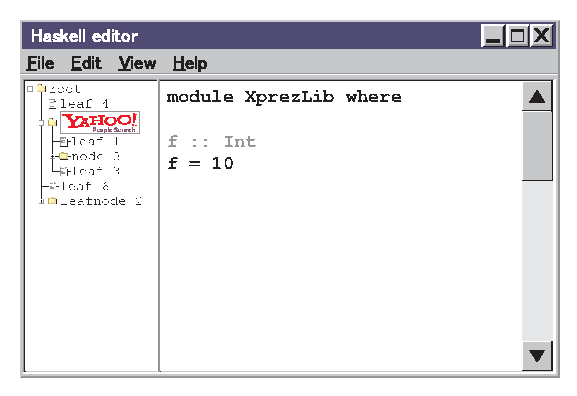
\epsfig{file=pics/eps/TreebrowserIntegrated.eps, height=4.5cm}\\ [2mm]
%??Tree-browser view
%\end{center}

%\editScreenshotTrns{$\langle$module structure + Haskell Editor$\rangle$}{$\langle$selected name has focus in %Haskell editor$\rangle$}{click on function name}

\begin{center}
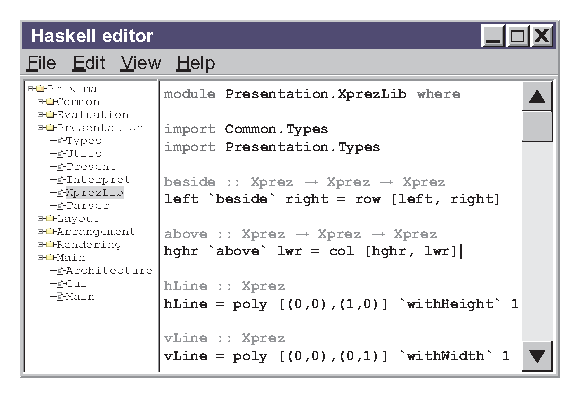
\epsfig{file=pics/eps/TreebrowserWindow.eps, height=4.5cm}\\ [3mm]
{\normalsize \sf  A source editor with a tree-browser pane.}
\end{center}


The window in the screenshot consists of two panes, the right-hand pane contains a Haskell source editor and the left-hand pane contains a tree view of the module structure of the edited program. \bc Below the module in the tree are the functions and types it defines.\ec When the user clicks on a name in the left-hand pane, the corresponding module is shown in the right-hand pane.

\head{Drag and drop}

The tree browser supports drag and drop edit behavior that allows nodes in the tree to be dragged to new locations. 

\begin{center}
\hspace{\stretch{1}}
\begin{tabular}[c]{@{}c@{}} %\\ [-2mm]
\fbox{\epsfig{file=pics/screenshots/TreeDrag.png.eps, height=3cm}}
\end{tabular}
\thenn
\begin{tabular}[c]{@{}c@{}} %\\ [-2mm]
\hspace*{0.8mm}\fbox{\epsfig{file=pics/screenshots/TreeDropped.png.eps, height=3cm}}
\end{tabular}
\hspace{\stretch{1}}\nopagebreak[4] \nopagebreak[4] \\ [3mm]
{\small move ``{\tt citrus}'' node}
\end{center}

%\editScreenshotTrns{$\langle$tree$\rangle$}{$\langle$rearranged tree$\rangle$}{drag tree node}

The screenshot shows the effect of dragging the node with label ``{\tt citrus}'' to a new position immediately below ``{\tt fruit}''. The operation results in a structural document change in which the element with presentation ``{\tt citrus}'' becomes the first child of the element that has presentation ``{\tt fruit}''.

In this example, the elements of the tree all have the same type and can therefore be moved anywhere in the structure. Using the tree view for outline editing in the word-processor example is slightly more complex, because a move operation may require a transformation of the element moved. For example, when a subsection is moved immediately under a chapter element, it must be changed to a section. 

\head{Customized tree views}

Because the tree presentation is not primitive, the editor designer or user can customize it, or even define entirely different tree presentations.


\begin{center}
\fbox{\epsfig{file=pics/screenshots/TreeAlternative.png.eps, height=1.9cm}}\\ [3mm]
{\normalsize \sf  An alternative tree-browser view.}
\end{center}
%\screenshot{
%\begin{tabular}[t]{lclclcl}
%	&+	&-Node	&-&-Leaf	& 	&\\
%	&\vline	&	&+&-Leaf	& 	&\\
%Root	&+	&-Node	&+&-Leaf	& 	&\\
%	&\vline 	&	&\vline&	&+	&-Leaf\\
%	&\vline 	&	&+&-Node	&+	&-Leaf\\
%	&\vline 	&	& &	&+	&-Leaf\\
%	&+	&-Leaf	& &	& 	&\\
%\end{tabular}
%}{}

The tree view in the screenshot is a more spacious presentation, in which the child nodes are presented to the right of the parent rather than below.


\head{Requirements} % tree browser

Similar to the equation editor, the tree browser has a two-dimensional graphical presentation that requires fine control over the alignment of the presentation elements. Customizability of the tree view requires that the presentation specifications are transparent and reusable. 

Edit operations on the tree structure are similar to edit operations on the table of contents in the word-processing example, because the tree is typically a derived structure that follows the structure of the document (or part of it). Updates on the tree need to be mapped on updates on the document itself. Navigation operations can be considered an update on the  focus and hence the specification formalism for document-oriented edit operations must support focus updates.

An aspect that is specific to the tree browser is that it has a notion of state. Each node in the tree view is either collapsed or expanded, and this information must be stored somewhere. Such presentation state, or {\em presentation extra state}, as we call it, does not form part of the document, because if it is stored there, the document type will need to be changed if a tree view is added to the presentation. The fact that this state is not part of the document, but rather of the presentation of the document, makes it hard to model in a structure editor. A mapping between the document and the presentation state needs to be maintained to associate a document node with its expansion state, even when the document is edited and its nodes are reordered. 


%																
\subsection{Simple tax form/spreadsheet}

The last example is a simple tax-form application, which is basically a spreadsheet with a rather specialized presentation. It contains questions and explanatory text, mixed with input fields and fields that contain derived information. 

\vspace*{1.4ex}
\begin{center}
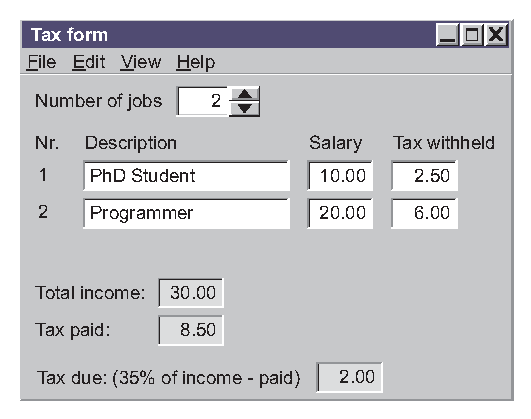
\epsfig{file=pics/eps/TaxWindow.eps, height=4.4cm}\\ [3mm]
{\normalsize \sf  A much simplified tax form.}
\end{center}
\vspace*{1.4ex}


%\screenshot{
%\begin{tabular}[t]{l@{\:\:}l@{\:\:}l@{\:\:}l}
%Income\\
%Nr. of jobs & \framebox(23,8){\hfill 2}\\
%\\
%Job nr. & Description & Salary & Tax withheld\\
%1 & \framebox(50,8){PhD student}		& \framebox(23,8){\hfill 10} &\framebox(23,8){\hfill 2}\\
%2 & \framebox(50,8){Programmer}	& \framebox(23,8){\hfill 20} &\framebox(23,8){\hfill 5}\\
%Total income:& 30\\
%Tax paid: & 7\\ 
%\\
%Interest:&\framebox(23,8){\hfill 2}\\
%\\
%Tax due:& \multicolumn{3}{l}{35\% of income - paid = {\bf 3.5}}
%\end{tabular}
%}{A much simplified tax form}


% Lambert:  income -> job income
%                job income = salary (??)

The tax-form editor has two different kinds of users: a user who designs the tax form, and a user who fills out the form. Both users use the same document type, albeit with different presentations. The form designer uses a presentation that shows the building blocks and structure of the form, as well as the formulas for the derived values. On the other hand, the user who fills out the form sees the input fields, the derived values, and the accompanying fragments of text. The structure of the form and the formulas for the derived values are not explicitly visible and cannot be modified in this presentation.

The distinction between the two kinds of users differs from the distinction in Section~\ref{sect:editing} between editor designer users and  document editing users, because for the tax form, both users edit the document and therefore are document editing users rather than editor designers.

A difference between the tax form and the previous use cases is that, similar to a spreadsheet, it has computations that are specified in the document itself. Hence, these computations can be modified by an editing user, rather than the editor designer. Although this is probably not how an actual tax-form application would be designed, we use the presence of computations in the document as an example of spreadsheet behavior in a structure editor.

%Navigating over form with subforms etc.

\head{Presentation depending on document values}

In most presentations, the structure of the presentation depends on the document structure. However, the presentation structure may also depend on a document value, rather than the structure. An example is the following section of the tax form:

\begin{center}
\hspace{\stretch{1}}
\begin{tabular}[c]{@{}c@{}} %\\ [-2mm]
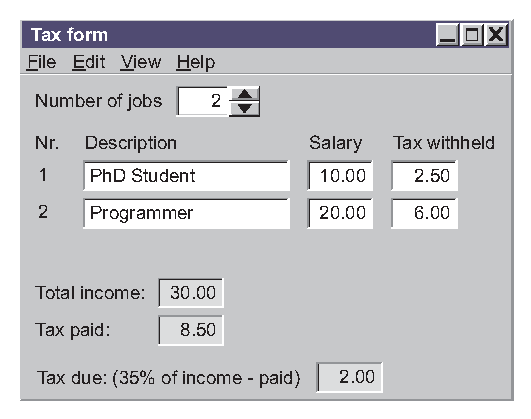
\epsfig{file=pics/eps/TaxWindow.eps, height=4.4cm}
\end{tabular}
\thenn
\begin{tabular}[c]{@{}c@{}} %\\ [-2mm]
\hspace*{0.8mm}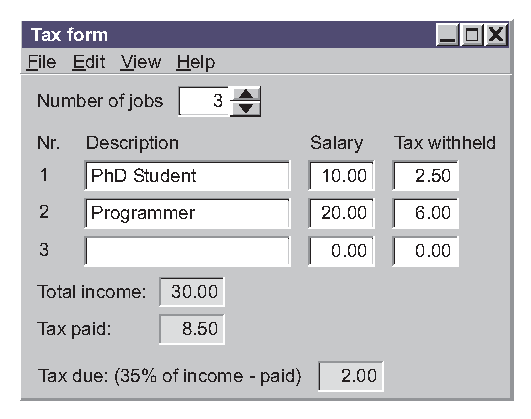
\epsfig{file=pics/eps/TaxWindow3.eps, height=4.4cm}
\end{tabular}
\hspace{\stretch{1}}\nopagebreak[4] \nopagebreak[4] \\ [3mm]
{\small increase number of jobs}
\end{center}


%\editScreenshotTrns{
%\begin{tiny}
%\begin{tabular}[t]{l@{\:\:}l@{\:\:}l@{\:\:}l}
%Income\\
%Nr. of jobs & \framebox(19,6){\hfill 2}\\
%\\
%Job nr. & Description & Salary & Tax withheld\\
%1 & \framebox(40,6){PhD student}		& \framebox(19,6){\hfill 10} &\framebox(19,6){\hfill 2}\\
%2 & \framebox(40,6){Programmer}		& \framebox(19,6){\hfill 20} &\framebox(19,6){\hfill 5}\\
%Total income: & 30\\
%Tax paid: & 7\\ 
%\\
%Interest:&\framebox(19,6){\hfill 2}\\
%\\
%Tax due:& \multicolumn{3}{l}{35\% of income - paid = {\bf 3.5}}
%\end{tabular}
%\end{tiny}
%}{
%\begin{tiny}
%\begin{tabular}[t]{l@{\:\:}l@{\:\:}l@{\:\:}l}
%Income\\
%Nr. of jobs & \framebox(19,6){\hfill 3}\\
%\\
%Job nr. & Description & Salary & Tax withheld\\
%1 & \framebox(40,6){PhD student}		& \framebox(19,6){\hfill 10} &\framebox(19,6){\hfill 2}\\
%2 & \framebox(40,6){Programmer}		& \framebox(19,6){\hfill 20} &\framebox(19,6){\hfill 5}\\
%3 & \framebox(40,6){}				& \framebox(19,6){\hfill 0} &\framebox(19,6){\hfill 0}\\
%Total income: & 30\\
%Tax paid: & 7\\ 
%\\
%Interest:&\framebox(19,6){\hfill 2}\\
%\\
%Tax due:& \multicolumn{3}{l}{35\% of income - paid = {\bf 3.5}}
%\end{tabular}
%\end{tiny}
%}{increase number of jobs}

The number of input fields for job information depends on the number of jobs. When the number is increased, the structure of the input form changes accordingly, showing an extra line of input fields. Decreasing the number hides the corresponding input fields, but after a subsequent increase, the fields reappear containing their previous values.

\head{The tax-man view} 

A different presentation of the tax form allows a user to design the form by editing the structure of the form, rather than the values of its input fields.

\begin{center}
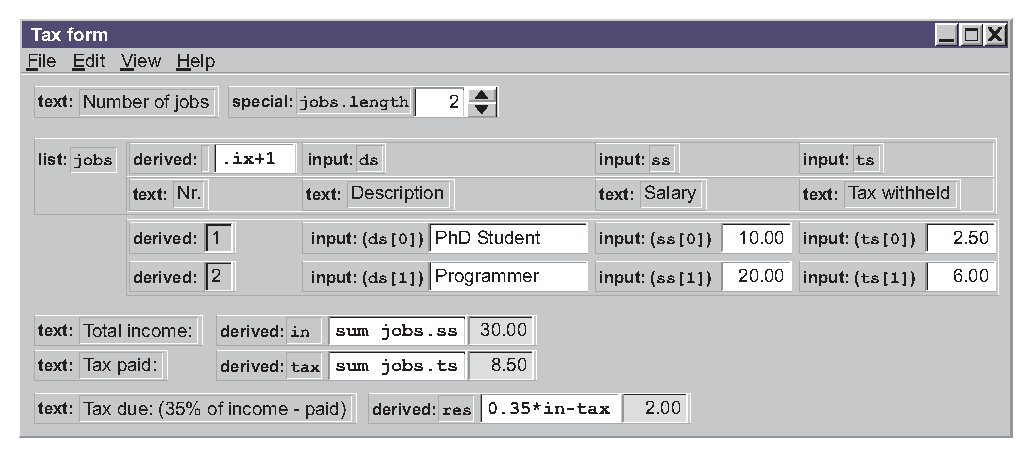
\epsfig{file=pics/eps/TaxMan.eps, height=5.25cm}\\ [3mm]  %4.9 is same size as 2->3 scrshot
{\normalsize \sf The tax form for the tax man.}
\end{center}
%\screenshot{
%\begin{tiny}
%\begin{tabular}[t]{l@{}|l@{}|l@{}|l}
%\framebox{Income}\\
%\framebox{Nr. of jobs} & c1: special \framebox{jobs.length}\\
%\\
%\framebox{Job nr.} & \framebox {Description} & \framebox{Salary} & \framebox{Tax withheld}\\
%LIST: jobs\\
%derived \framebox {index} & cs1: input & cs2: input & cs3: input \\
%derived:  1 & cs1[0]: input \framebox{PhD student}		& cs2[0]: input \framebox{10}& cs3[0]: input %\framebox{2}\\
%derived: 2 & cs1[1]: input \framebox{Programmer}	& cs2[1]: input \framebox{20}& cs3[1]: input \framebox{5}\\
%\framebox{Total income:} & c2: derived \framebox{sum cs1} {\em 30}\\
%\framebox{Tax paid:} & c3: derived \framebox{sum cs2} {\em 7}\\ 
%\\
%\framebox{Interest:}& c4: input \framebox{2}\\
%\\
%\framebox{Tax due:}& \multicolumn{3}{l}{
%\framebox{35\% of income - paid = }
% \vline\ c5: derived \framebox{0.35*(c2+c4)-c3} {\bf \em 3.5}
%}\\
%\end{tabular}
%\end{tiny}
%}{Tax form for the tax man}

The screenshot gives an impression of a presentation in which the tax-form structure and layout are editable. The tax-form document is the same as for the first screenshot. Text blocks, as well as input fields and derived value fields can be inserted or deleted, and the computations for the derived values (``{\tt .ix+1}'', ``{\tt sum jobs.ss}'', ``{\tt sum jobs.ts}'', and ``{\tt 0.35*in-tax}'') can be modified. \bc The labels (c1 \dots c5, and cs1 \dots cs3) are supplied automatically, but may also be changed. \ec The input values of the input fields are still editable to allow for easy testing of the specified computations. 



\head{Requirements} % tax form

In contrast to the other use cases, the tax-form presentation is rather similar to a user interface. Instead of just text and graphical elements, it contains widgets, such as check boxes, selection lists, and input fields, with the corresponding edit behavior.

The tax form also features computations with results that appear explicitly in the presentation itself. Unlike the type computations in the Haskell editor, the computations in the tax form are part of the document, and may be specified by an editing user (the tax man), rather than an editor designer. Therefore, similar to a spreadsheet application, the editor needs to dynamically interpret document structures that represent computations and display the results in the presentation. 

%																
%																
%																
\section{Functional requirements} \label{sect:reqs}

With the use cases of the previous section in mind, we now provide a number of functional requirements for a generic structure editor. 


%																
\subsection{Genericity}

The primary requirement for the editor is genericity: the editor must be generic in the sense that it is not built for a specific document type or class of document types. However, as mentioned in Section~\ref{sect:structdocs}, we restrict ourselves to trees rather than graphs. Most documents can be represented by trees, including our five use cases. A formalism for specifying cross-links between tree nodes is desirable, but full graph editing is not a requirement.

%Although a distinction can be made between editor generators and generic editors, we regard both as generic editors.


%																
\subsection{Computation formalism}

An interesting aspect of an editor that has knowledge of the structure of the document, is that it can show derived values over that structure to the user. Examples of derived values are chapter numbers and a derived table of contents, but also derived type information for a program source. An important point is that the computations we refer to are part of the presentation process. Based on values in the document, the derived value is computed, but the document itself is not affected. This is different from computations that map the document onto a new document containing derived values. The latter kind also allows computed values to be shown to the user, but in the process causes an update to the document. Hence, we view such computations as document-oriented edit operations, which are covered by the {\em editing power} requirement, discussed in Section~\ref{sect:editingPower}.


Two aspects influence the usefulness of the computations: the expressivity of the formalism in which the computations are specified, and the integration of computed values and structures with the document presentation. 
%\todo{integration very low (separate window) means that doc edit ops are almost computations}

% or connection to something

For program editing as well as the tax form, the expressivity of the computation formalism is important. Computations can provide static analysis, e.g.\ detecting name clashes and scoping problems, as well as a type derivation. In order to be able to specify these computations for arbitrary languages, a Turing-complete formalism, such as an attribute grammar~\cite{swierstra04ag}, is desirable. Other options include constraint-based systems~\cite{ganzevoort92views,myers90garnet,borning81thinglab,ballance92pan} \bc christopher90constraints \ec and tree transformation formalisms~\cite{visser01stratego,xslt10}. Furthermore, the computation formalism should offer functionality for connecting to external tools, such as a compiler or a theorem prover.

For the word-processing example, as well as the tax form, the integration of computed values with the document presentation is important. Whereas type errors may be shown in separate windows or by underlining the location and showing the message in a tooltip, chapter numbers and a table of contents form an actual part of the presentation. 



%																
\subsection{Presentation formalism} \label{sect:presentationFormalism}

The presentation formalism has two different aspects, which we consider together here. One is the formalism in which the building blocks of the presentation are expressed (the {\em presentation target language}), whereas the other  (the {\em presentation specification language}) is the formalism in which it is specified how a document is mapped onto an element of the presentation target language. For XML, a well-known presentation language is the Extensible Stylesheet Language (XSL)~\cite{xsl10}. XSL is split into the mapping language XSLT~\cite{xslt10} and the target language XSL Formatting Objects. Chapter~\ref{chap:presenting} discusses presentation languages in more detail.

In many editors the {\em presentation target language} consists of just plain text, sometimes with color and font attributes. However, in order to support the graphical presentations of the equation editor and outline view use cases, a more advanced target formalism is required. It must be possible to specify graphical elements such as lines and boxes, as well as to show images. Furthermore, the presentation of a mathematical formula requires an advanced alignment model that offers full control over the positioning of presentation elements.

Another requirement for the presentation target language comes from the tax-form example. The tax form typically contains user-interface widgets, such as buttons, selection lists, and menus. Therefore, the target language must support user-interface widgets.
% The presentation language may provide built-in support for such widgets, but if  the language
% is powerful enough, they may also be emulated.


Finally, the word-processor use case requires that the presentation target language supports line and page breaking, preferably optimal~\cite{knuth82breaking}. 

The {\em presentation specification language} has to allow the specification of complex graphical presentations using compact readable style sheets. It must be possible to specify simple presentations in an easy way, while still allowing the specification of more complex presentations. For the exact choice of formalism we have similar options as for the computation formalism, including AGs, constraint-based systems, and tree transformation formalisms.

Although a presentation can be seen as a computed value, we make a separation between the presentation specification language and the computation formalism. One of the reasons is that the separation of computation and presentation makes it possible to specify multiple presentations of a document together with its computed values. Furthermore, the separation makes it easier to support edit operations on derived structures.


%																
\subsection{Editing power} \label{sect:editingPower}

The editing power of an editor is determined by the fact whether both document- and presentation-oriented editing is supported, together with the complexity of the edit operations and to what extent these operations are user-specifiable. 

%Levels at which editing is possible are the presentation and the document. Furthermore, as we will show in %Chapter~\ref{chap:proxArch}, a number of other levels may be distinguished, among which a level that contains derived %structures and values.


% document-oriented editing
The equation editor as well as the outline editor rely heavily on document-oriented editing. Document-oriented edit operations typically include basic copy, paste, and delete operations, as well as selection and navigation operations.

Because a document is not always well typed while it is being constructed, the editor should support incomplete document structures, for example by allowing placeholders to appear in the document tree. Besides incomplete documents, it is desirable to have support for invalid documents in general. However, because it can be difficult to compute the presentation of an invalid document, we may wish to allow invalid documents only for certain presentations, such as a textual XML source presentation. 

%presentation-oriented editing
Presentation-oriented editing is required for the source editor, because it supports free textual editing of the program source. To a lesser extent, presentation-oriented editing is needed also for the equation editor (for textual structure entry) and the tax form (for editing the computations). 

Finally, as the editable table of contents of the word processor use case shows, support for edit operations on derived structures is desirable. This is not to say that all derived structures and values should be editable, but in those cases in which it makes sense to a user, it should be possible to specify the edit behavior for derived structures.
% say more? that is should be easy to do standard stuff?

For document-oriented edit operations, a transformation specification formalism is desirable. It allows an editor designer to define edit operations specific to a certain type of document. An example of such an edit operation is the rename operation in the Haskell editor. Furthermore, the formalism can be used to specify standard generic document-oriented edit operations such as split and join.


%																
\subsection{Modeless editing}

Besides support for both document- and presentation-oriented editing, an important requirement is the integration of these two kinds of editing. A seamless integration provides a pleasant edit interface to the user, as the intended operation can be performed on the presentation the user is working on, without first having to explicitly switch modes. In case an edit operation is a meaningful operation on both the document and the presentation (yielding different results), the editor can give preference to the document operation, with the possibility to override this preference. Sufrin and De Moor describe a basic modeless structure editor~\cite{sufrin99modeless}, but the idea of modeless editing is also found in earlier publications (e.g.\ Kaiser and Kant~\cite{kaiser85parsingWithoutParser}).

The most extreme form of mode-switching is when edit operations on different levels have to take place in separate windows and also have a separate undo-history. This is the approach taken by many pure structure editors that offer some support for free text editing, as well as by all existing XML editors. Even worse, the separate free-editing text mode often has a special text-only format, in which derived values are not shown and interesting graphical presentations are not possible. In order to get back to document-oriented editing, the user needs to leave the text in a valid state, or abandon the text update.
%\pagebreak

If the editable textual presentation is displayed in-place in the document presentation, the mode-switching becomes less intrusive. However, the most user-friendly approach is to avoid mode switching altogether, thus allowing a user to freely edit the presentation, even if it contains computations and graphical presentations. Moreover, if a presentation-oriented edit operation makes the presentation invalid, the invalid area should be kept as small as possible, and document-oriented editing must still be available on the valid parts.


%																
\subsection{Extra state} \label{sect:editingExtraState}

If a document is edited, the presentation is updated accordingly by presenting the modified document. In some cases, however, a presentation may contain information that cannot be derived from the document. We refer to such information as {\em presentation extra state}. Analogously, the document may contain information that cannot be inferred from the presentation. This information is referred to as {\em interpretation extra state}. 

A clear example of {\em presentation extra state} is found in the outline view example. The expansion state of the nodes of the tree view needs to be kept track of. However, this is not information that should be stored in the document tree structure, since the design of the document type should not have to consider what views may be defined for that document type. Moreover, several views may be opened simultaneously, each with their own expansion state. Hence, the expansion state is regarded as presentation extra state. Other examples of presentation extra state are focus information, local layout settings (e.g.\ whether or not auto-layout is turned on), and whitespace in the presentation. 

{\em Interpretation extra state}, on the other hand, is any information in the document that cannot be inferred from its presentation. Hence, if a document is only partially presented, those parts that are not presented are considered interpretation extra state. An example is an editable table of contents of a word processor, in which the content of the chapters and sections is interpretation extra state.

In order to handle the use cases, a generic editor should support both presentation extra state, and interpretation extra state (in the form of editable partial presentations). We do not consider a generic editor to fully support presentation extra state if it only supports a built-in form of it. Instead, it must be possible to explicitly declare parts of the presentation to be extra state.

\bc
The examples all concern extra state at presentation level, but extra state also appears on other levels, as will be shown in Chapter~\ref{chap:proxArch}. In order to handle extra state, a formalism must be present to declare variables local to presentation elements. Furthermore, when a document is stored, its extra state must also be stored as well. **** also mention interpr. extra state + \ref{sect:extraState}
\ec

In order to support extra state, an editor needs to maintain information about the mapping between the document and its presentation. If there is no extra state, no extra effort should be required from the editor designer. Extra state is discussed in more detail in sections~\ref{sect:extraState} and~\ref{sect:singleExtra}

\bc
Support for extra state complicates the presentation process as well as the interpretation process. A document element needs to keep track of its presentation elements, and when it is re-presented, it must be mapped onto those same presentation elements because extra state may be associated with the presentation. Similarly, the presentation elements must keep track of the document . The editor needs to have facilities for keeping track of the information required to support extra state, and
\ec


%																
\subsection{Summary}

Summarizing, to support all five use cases, a generic structure editor must meet the following requirements.

\begin{itemize}
\item Genericity.
\item Support for any computation over the document.
\item A graphical presentation language with a powerful mapping formalism.
\item Support for both presentation-oriented and document-oriented editing %, including edit operations on derived structures.
\item Modeless editing.
\item Support for presentation extra state as well as interpretation extra state.
\end{itemize}

The requirements above all apply to the edit model, but of course many other requirements exist for a generic structure editor.  Commonly recognized requirements for editors, which we will not discuss in detail, include: undo functionality, multiple window support, search/replace functionality, and a help facility. 
%macro language?

%The computation model of Proxima is general, and in order to easily use it for example to do semantic analysis or code %generation, libraries are required. Furthermore, there are requirements that we consider.
%Furthermore, requirements that we consider orthogonal to ours, concern document management and database connectivity. 
\bc
more?
The discussed concepts are mainly related to the edit model of the system. 
Document model and edit model. Not things like multiple window, XSL output feature etc.
Mention that these requirements are different from things like multiple window, XSL output window, help feature, etc. Those are added easily, no specific model needed. Requirements here are more fundamental.

plug-in architecture, open.
%somewhere:
lso focus on single documents (although not hard) 
instead of document management, versioning, or compound documents. Mainly orthogonal.
page refs are a bit tricky.
\ec







%																
%																
%																
\section{Overview of structure editors} \label{sect:editorOverview}

Because of the large number of existing systems, we can only mention a selection of editors in this overview. The editors mentioned are some of the early systems, together with a number of other editors that contain novel features.


It is important to note that the systems are discussed with the requirements from Section~\ref{sect:reqs} in mind. If an editor does not meet our requirements or has been left out of the discussion, this does not necessarily say anything about the quality of that system. Many generic editors were designed to support  a particular class of editor applications (e.g.\ program editors) rather than the entire range of use cases from Section~\ref{sect:usecases}. Moreover, many of these systems have interesting features that are orthogonal to our requirements, and the techniques for supporting these features may be applicable to Proxima editors as well.


\bc
that many of these systems were designed with a more specialized purpose?. Hence, most editors only meet a few of our requirements. ALso left out does not mean bad. Many structure editors have interesting features for their domain. 

Nevertheless, even though not suitable for implementing the use cases, the mentioned systems may have unique features.  
Important point.
Many are program editors, with unique features, but not suitable for our use cases. Nevertheless, research in many cases orthogonal and parsing techniques may be applicable to Proxima editors as well.
\fromHere
\ec

%																
\subsection{Syntax-directed editors} \label{sect:synDirEditors}

Most of the editors in this section are specifically designed for program editing and hence have a rather text-oriented presentation formalism. Moreover, the computation formalism in such editors is aimed mainly at analyzing source code, and not at performing general-purpose computations. 

Most syntax-directed editors allow partial presentations of the document, and hence offer support for interpretation extra state. On the other hand, presentation extra state is only found in built-in tree views on the document structure.

\head{Synthesizer Generator}

The Synthesizer Generator~\cite{reps84synGen} is the successor of the Cornell Program Synthesizer~\cite{teitelbaum81progSynth}, one of the early syntax-directed editors. Because the system is targeted at programming languages, the presentation is simple and text-only, although newer versions have some font and color control. 

%prog Sys is monolithic, also for program execution.

An interesting aspect of the Synthesizer Generator is its support for computations over the document structure. The presentation of the document can contain computed values, which are specified using an attribute grammar. 

The edit model supports user-specified transformations on the structure, but plain text editing is poorly supported. The editor uses mode-switching, and after switching to the textual mode, the presentation must be left in a parsable state before structure editing is available again.

Over the years, the behavior and design have not undergone many drastic changes, but the system is still being used and commercially maintained.

\head{LRC}

The LRC attribute-grammar system~\cite{saraiva00lrc} was a research project at Utrecht University. Higher-order attribute grammars are used to specify the derived values, as well as the presentation. The system is based on an efficient higher-order attribute-grammar evaluator. Higher-order attribute grammars allow some computations to be specified more elegantly than regular attribute grammars.

For the presentation of the document, the Tcl/Tk language is used. This allows for complex presentations with multiple windows, GUI widgets, colors, and basic graphical elements. However, the integration between the generated presentation and the editor is rather weak. No general focus model is present, and although edit events can be attached to the Tcl presentation, free editing is only possible in a separate window that contains a purely textual presentation of the document. The textual presentation cannot be used to edit the layout of the main presentation, and it does not contain derived values. 

\head{SbyS, Mj\bfslasho lner/Orm} %90

SbyS is the structure editor of the Mj\slasho lner/Orm environment~\cite{magnusson90orm}. Mj\slasho lner/Orm is a generic language and software development environment. An interesting aspect of the environment is that it is truly a generic environment, since language descriptions can be changed without the need to recompile or regenerate the editor. In contrast, most of the other systems are editor generators.

SbyS supports textual editing only for entering expressions. In order to overcome the usability problems associated with pure syntax-directed editing, the editor employs the concept of direct manipulation. Program constructs are shown in a palette, from which they can be dragged to the program source or a clipboard.

No formalism for specifying transformations is present, and the only computations that can be specified are aimed at semantic analysis and code generation. Derived values cannot be part of the presentation.


\head{PSG} % 86

PSG (Programming System Generator)~\cite{Bahlke86PSG} is a generator for language-based interactive environments, developed at the Technical University of Darmstadt. As the name suggests, the system is designed for programming languages. The presentations are text-only, and only LL(1) grammars are supported. The system generates an editor based on a number of formal descriptions for a language, including a syntax definition, a presentation sheet (called a {\em format syntax} in PSG), and a specification of the semantic analysis.

Special focus has been put on incremental analysis over incomplete program fragments. PSG uses a special form of the attribute-grammar formalism that supports sets of possible attribute values in order to handle attribution of incomplete document fragments.

However, the presentation may not contain derived values or structures. And although textual editing takes place in the same view as document-oriented editing, this does involve a mode switch. Furthermore, layout information cannot be edited freely, but is determined by the presentation sheet.

\head{Other syntax-directed editors} % 86

% mention text only syn-dir editors with parser mentor
Other textual syntax-directed editors for program editing are the Aloe editor in Gandalf environment\cite{notkin85gandalf}, Mentor~\cite{donzeau84mentor}, its successor Centaur~\cite{borras88centaur}, Pregmatic~\cite{brand92pregmatic}, Poe~\cite{fischer84poe}, Dose~\cite{kaiser88dose}, Gnome~\cite{garlan84gnome}, Pecan~\cite{reiss84pecan}, Muir~\cite{normark88muir}, and Dice~\cite{fritzson84dice}. These systems have their own interesting aspects, but as far as the editors are concerned they do not deviate much from the systems already discussed, and hence are not discussed separately.
%Cedar?   http://portal.acm.org/citation.cfm?id=801968&dl=ACM&coll=portal#
Some more exotic editors that do not support editing on the presentation are Multiview~\cite{read96multiview} and {VL-Eli}~\cite{kastens02vl-eli}.


%																
\subsection{Syntax-recognizing editors}

Similar to the syntax-directed editors, most syntax-recognizing editors are designed for program editing. Regarding the computations, however, due to the difficulty of free editing in a presentation with derived values, none of the syntax-recognizing editors support arbitrary computations that may appear in the presentation.
%\pagebreak

Regarding extra state, syntax-recognizing editors are the opposite of syntax-recognizing editors: several built-in forms of presentation extra state (e.g.\ whitespace) are supported, but interpretation extra state is not. 

\bc
\toHere     % ^^^^^^^^^^^^^^^^^^^^^^^^^^^^^^^^^^^^^

% More Presentation oriented
\head{SRE}\\

No information on this one yet. Order paper at library.

\fromHere  % VVVVVVVVVVVVVVVVVVVVVVVVVVVVVVVVVVVVVVVVVVVV
\ec

\head{Pan}

Pan~\cite{ballance92pan} is a text-only source editor environment. The presentations are text in multiple fonts, styles, and colors. The system has good support for handling partially incorrect or incomplete documents.

The computation formalisms in Pan are oriented towards semantic analysis. Logical constraint grammars are used for specifying, checking, and maintaining contextual constraints. Computed information is shown in the presentation by changing the font and color attributes of the text, but it is not possible to specify arbitrary computations that form part of the presentation. Furthermore, the editor does not support interpretation extra state. Hence, it is not possible to specify an editable presentation that shows only part of the document (e.g.\ a presentation in which function bodies may be hidden), as the editor is syntax-recognizing, and therefore the presentation must contain all information necessary to derive the document structure.

Pan offers some document-oriented editing, but edit operations on document structures are performed by editing the corresponding parts in the presentation and reparsing the presentation. Edit operations that modify the document structure directly are not supported, as these are believed to confuse the user. As a consequence, only basic document-oriented edit operations such as cut and paste are supported, and no document transformations can be specified. Free text editing, on the other hand, is fully supported, including layout editing. 

\head{GSE, ASF+SDF}

\bc
The GSE~\cite{koorn92gse} editor has been developed as part of the Esprit project ``Generation of Interactive Programming Environment'' (GIPE). It is still being used in the ASF+SDF meta environment~\cite{klint93asfsdf}. The editor is primarily aimed at programming languages and the presentations are assumed to be lines of text. GSE supports free editing of the program text without an explicit mode switch, but structural edit operations on the program that keep user-specified layout intact are not supported. Furthermore, the results of computations on the document cannot be shown in the presentation. \ec

The GSE~\cite{koorn92gse} editor has been developed as part of the Esprit project ``Generation of Interactive Programming Environment'' (GIPE). It is part of the ASF+SDF meta environment~\cite{klint93asfsdf} and under active development. The editor is primarily aimed at programming languages and the presentations are assumed to be lines of text. GSE supports free editing of the program text without an explicit mode switch. A powerful transformation formalism is available for specifying document edit operations that keep intact the layout~\cite{brand00rewriteLayout}. On the other hand, such transformations cannot form part of the presentation process.


\head{Ensemble}

The Ensemble project is a successor to Pan, based on the recognition that structure editing cannot only be used for program editing, but also for editing documents of a more graphical nature, such as documentation. The system handles compound documents containing subdocuments of different types, and provides document management functionality, such as versioning.

Ensemble specifies formalisms for performing incremental semantic analysis, but arbitrary computations appearing in the presentation cannot be specified. However, some support for derived structures is present in the presentation formalism.

% check tree transformation formalism
Ensemble has a powerful graphical presentation formalism, including a constraint-based box layout. The presentation specification language, however, does not elegantly allow presentations with a structure different from the document. The presentation formalism may be used to specify derived structures, but these are not editable.

The edit model supports modeless free text editing, including layout editing, as well as structural editing.

The Ensemble project has been terminated, but its successor, Harmonia~\cite{boshernitsan01harmonia}, is still under development. Because the monolithic character and ambitious design requirements of Ensemble slowed down its development, Harmonia is a framework for incremental language analysis rather than a single editor generator. The services from Harmonia can be used to augment text editors, such as Emacs, with language-aware editing and navigation functionality.

\head{Desert}
%S. Reiss. FIELD: A Friendly Integrated Environment for Learning and Development. Kluwer %Academic Press, 1994.

Built with the experience of the FIELD~\cite{reiss94field} project, Desert~\cite{reiss99desert} is a syntax-recognizing editor generator that uses the commercial editor system Framemaker for editing program sources. The system has many facilities for software development, including database facilities and an interface for easily defining (non-editable) software visualizations. The actual editor is a syntax-recognizing editor with attributed text and images in the presentation. However, no structural edit operations, or derived structures in the presentation are supported.

\head{Other syntax-recognizing editors}

Other syntax-recognizing editors similar to the ones that were discussed include  Babel~\cite{horton81babel}, Saga~\cite{campbell84saga}, and Pregmatic~\cite{brand92pregmatic}.


\bc
CodeProcessor~\cite{codeprocessor}
Lapis, text only

\head{Intentional Programming Editor}
Interesting structure editor with powerful presentations, discontinued, little publications on
internals. Monolithic system, program oriented. Transformations. No evidence of full 
integrated computations. Edit model mimics text editing, but apparently no integrated
both level editing
\ec


%																
\subsection {Editor toolkits} \label{sect:toolkits}

Besides generic editors and edit generators, an editor can also be built using an editor toolkit. The toolkit is a collection of libraries and tools that can be used when building an editor. The editor application itself, however, has to be written by hand. The distinction between a toolkit and a generator is not always completely clear, since the specifications that an editor generator uses for specifying language, presentation, and semantics can be considered programs as well. The toolkits we consider here all require a substantial amount of programming in order to build an editor.

The advantage of a toolkit is that the final editor can be customized to a high degree, but this comes at the cost of the increased effort required for building an editor. 

\head{Amaya, Thot}

Amaya~\cite{amaya04} is the W3C web browser that is built on top of the editor toolkit Thot\cite{quint97thot}, which is a successor of Grif~\cite{quint86grif}. The Thot toolkit supports a number of specification languages for document structure, presentation, and transformation, but in order to build an actual editor C code is required to connect the various components.

The presentation formalism in Thot, called P, is a powerful graphical presentation formalism, somewhat similar to Proteus (Ensemble), but with more advanced alignment features. As a result, complex presentations are possible, such as the presentation for the equation editor use case.

Thot editors are of a syntax-directed nature. Multiple views on the document may be edited simultaneously, and user-specified transformations are supported. However, free text editing can only be done in a separate window in a different mode. Also, no computations are supported other than some basic counters in the presentation. 

%\head{Eclipse}
%
%\cite{eclipse2001}
% IDE, also editor Program editor.
%veel programmeerwerk.
%
%***{also add to comparison}

\head{Visual Studio editor}

The Microsoft Visual Studio environment includes an integrated source editor. Although the editor does not contain any novel features, and thousands of lines of code need to be written to tailor the editor for a specific language, we do include it in the discussion because it is a structure editor that is actually used by a rather large number of people. 

The Visual Studio editor is of the syntax-recognizing kind with colored-text presentations. No document-oriented edit functionality is supported, other than performing semantic analysis and displaying the results. These results are displayed by marking a location in the source with a squiggly \makebox(0,0)[lt]{
\epsfig{file=Pics/eps/squiggly.bmp.eps, width=0.042in}
\epsfig{file=Pics/eps/squiggly.bmp.eps, width=0.042in}
\epsfig{file=Pics/eps/squiggly.bmp.eps, width=0.042in}
\epsfig{file=Pics/eps/squiggly.bmp.eps, width=0.042in}
\epsfig{file=Pics/eps/squiggly.bmp.eps, width=0.042in}}line, and displaying a corresponding message in a separate window pane as well as in a tooltip. Pop-up list boxes can be used to show auto-completion alternatives. Despite its simple model, in which semantic analysis is only possible when the entire presentation is syntactically correct, the editor provides a surprisingly usable environment. 

\bc
\toHere     % ^^^^^^^^^^^^^^^^^^^^^^^^^^^^^^^^^^^^^

\head{Other editor toolkits}

*First find out more about them.*\\
Xemacs\\
Andrew system\\
Opendoc.\\

\fromHere  % VVVVVVVVVVVVVVVVVVVVVVVVVVVVVVVVVVVVVVVVVVVV

% FIELD? and its relation to Desert?

% what about non source editors? mention, ref, ignore?
\ec

%																
\subsection{XML editors} \label{sect:xmlEditors}

A large number of XML editors have been developed, but the differences between them are not fundamental. Almost all XML editors classify as pure structure editors with mode switching. 

Because the differences are small, we discuss XML editors in general with respect to our functional requirements. Afterwards, two  editors are discussed separately.

\begin{description}
\item[Genericity.] 
The XML editors are generic. Most reviewed editors are actual generic editors, rather than editor generators, and support editing of documents with arbitrary DTDs. Although, compared to context-free grammars, DTDs have a few restrictions in order to make parsing easier~\cite{klein98glushkovRestr}, the type language is very similar to the EBNF grammar description formalism and powerful enough to describe the tree-based document structures we wish to edit.

\item[Computation formalism.]
Support for computations is very weak for all reviewed editors. A few editors support basic numbering of elements in the document, but no arbitrary computations can be specified. Some editors support the transformation formalism XSLT, but none provide an editable view on the resulting transformed document.

\item[Presentation formalism.]
Most XML editors only provide standard views on the document. Popular are the raw-text XML source view, a built-in tree view showing the document structure with the textual content in the leaves, and a slightly less raw view with tags, represented using a more graphical presentation.

Some editors support a user-defined presentation, or at least allow the user to specify some attributes for the presentation. However, the presentation formalisms are generally weak, and the presentations that can be used for editing have to follow the structure of the XML document. Moreover, there is hardly any support for textual presentations, making it impossible to present an XML tree that represents an abstract syntax tree as actual program source code.

It is remarkable that support for textual presentations of XML documents is this weak, since many languages for processing and describing XML documents are specified in XML itself (e.g.\ XML Schema~\cite{xmlSchema1,xmlSchema2}  and XSLT~\cite{xslt10}) and editing these languages would be greatly simplified by providing the user with a concise concrete syntax, rather than the verbose XML syntax.

\item[Editing power.]
%check transformation
Most XML editors offer simple document-oriented edit operations for structure entry and manipulation. However, none of the reviewed editors support user-specified transformations on the tree structure.

In each of the editors, free text editing is supported only in the raw XML source. Because most XML documents have text and whitespace in the leaves, it may appear that the document-oriented edit operations are free text editing, but this is not the case. Textual presentations other than the source presentation cannot be edited freely. On the other hand, as mentioned, most XML editors offer little support for textual presentations of the document. 

\item[Modeless editing.]
None of the editors support free editing on the presentation without a mode switch. Each type of view has a separate window, and though some editors have a shared undo history for some of the views, no editor has a shared undo history for the XML source presentation and its other presentations. Hence, after switching to source mode, previous edit operations on other views cannot be undone, and vice versa.

\item[Extra State.]
The XML editors support extra state similar to the syntax-recognizing editors. Interpretation extra state is supported in the form of partial presentations, but presentation extra state is only found in built-in tree views.

\end{description}

Two XML editors have a more sophisticated presentation engine and basic support for computations, and are therefore discussed separately.

\head{X-Metal}

The commercial system X-Metal from SoftQuad is a highly customizable XML editor, with support for many XML standards and database connectivity. Besides regular source and outline views, it offers built-in table editing and an editable CSS~\cite{css2} presentation of the document. CSS provides a quick and easy way to specify a document presentation, but its expressive power is limited. Although general computations cannot be specified, CSS does allow the specification of basic counters in the presentation. 

Document-oriented edit operations in X-Metal are rather weak, and transformations cannot be specified. Furthermore, the freely editable source presentation can only be edited in a separate mode.

% mention frame maker here?
\head{XMLSPY}

XMLSPY is a large system that has functionality similar to X-Metal. An important difference is the presentation system. XMLSPY supports a larger number of built-in presentations and also supports a user-defined presentation definition for the specification of simple derived structures. Values from the document that appear in the derived structure may be edited in place, but the structure itself is not editable.

%\head{Frame maker?}\\


\section{Discussion} \label{sect:discussion}

% Also a number that were not introduced due to space limitations (or some similar reason)?

\begin{figure}
\begin{center}
\begin{scriptsize}
\begin{tabular}[t]{l|c|c|c|c|c|c}
 			&Genericity& Computation & Presentation & Editing    & Modeless & Extra \\
			&		&   formalism   &   formalism   & power     &  editing   & state \\
\hline
%                                           generic  comps      pres        editing    integration extra state
Synthesizer Generator	&  $++$	&   $++$	&  $\pm$ 	&   $+$	&   $--$	&    $\pm$ 	\\
LRC					&   $++$	&   $++$	&   $+$ 	&   $+$	&   $--$ 	&    $\pm$	\\
PSG					&   $++$	&    $+$	&   $--$	&   $\pm$	&  $+$	&    $\pm$	\\
SbyS \bc, Mj\slasho lner/Orm\ec&   $++$	&   $-$	&   $--$ 	&   $-$		&   n/a	&    $\pm$	\\
\hline
%SRE			&   ?	&   ?	&   ? 	&   ?	&   ?	&    $--$	\\
Pan					&   $++$	&  $\pm$	&   $-$ 	&   $\pm$	&   $++$	&     $-$	\\
GSE					&   $++$	&   $--$	&   $--$ 	&   $+$		&   $++$	&     $-$	\\
% GSE layout structure edit: \pm to +      and    whitespace es: - to pm?
Desert				&   $++$	&   $--$	&   $\pm$ 	&   $\pm$	&   $--$	&     $-$	\\
%Intent. Progr. Editor	&   ?	&   ?	&   + 	&   ?	&   $++$	&    $--$	\\
Ensemble				&   $++$	&   $\pm$	&   $+$ 	&   $+$	&   $++$	&     $-$	\\
\hline
Amaya, Thot			&   $+$	&   $\pm$	&  $+$ 	&   $+$	&   $--$	&    $-$	\\
Visual Studio			&   $\pm$	&   $\pm$	&   $-$ 	&   $-$	&   n/a	&    $-$	\\
\hline
XMetal				&   $++$	&   $-$	&  $\pm$ 	&  $\pm$	&   $--$	&   $\pm$	\\
XMLSPY				&   $++$	&   $\pm$	&   $+$ 	&  $\pm$	&   $--$	&   $\pm$	\\
Other XML editors		&   $++$   & max. $-$ & max. $\pm$&  $\pm$&   $--$	&   max. $\pm$	\\
\hline
%\dots			&   ?	&   ?	&   ? 	&   ?	&   ?	&     $-$$-$	\\
Proxima				&   $++$	&   $++$	&   $++$ 	&   $++$	&   $++$	&     $++$	\\
\end{tabular}                                                   
\end{scriptsize}
\caption{Editor comparison}\label{scoretable} 
\end{center}
\end{figure}



%             EXPLANATION OF SCORES??
 
\bc
More flexibility, more freedom. More power, so less disadv. and more adv. An overview of existing structure editors is given, together with an evaluation according to the requirements. 

\section{Problems with current editors}
An xml editor for Haskell would never be possible
\begin{itemize}
\item No computation formalism
\item Presentation formalism too weak. 
\item No extra state support. layout, treebrowser expansion
\item Mode switching editors hard to use
\item Either text only, or no free editing
\end{itemize}
\ec

Figure~\ref{scoretable} contains an evaluation of the strengths and weaknesses of each of the discussed editors according to the requirements from Section~\ref{sect:reqs}. None of the editors scores a positive for extra state, and besides that, each of the editors has at least one or more columns with a low score ($\pm$ or less). 

The reason why no editor scores positive on the extra state requirement is that, although it is rather straightforward to support either presentation or interpretation extra state, it is hard to support both forms. A syntax-directed editor without support for presentation-oriented editing may support interpretation extra state simply by ignoring it during presentation. Similarly, a syntax-recognizing editor without document-oriented editing may support presentation extra state by ignoring it during interpretation. The syntax-recognizing editors score lower on extra state than the syntax-directed editors because only built-in forms of presentation extra state are supported, whereas the interpretation extra state for the syntax-directed editors may be specified by the editor designer.

The main reason why no editor has a line containing only positives is that the requirements for the computation and presentation formalisms interfere with the requirements for editing power and modelessness. The former two requirements determine the presentation complexity of the editor, whereas the latter determine the usability of the editor. A problem is that the more complex a presentation is, the harder it will be to still offer modeless free editing on the presentation level.

{\bf Syntax-directed editors.}~\,The syntax-directed editors tend to do well on the computation requirement, but at the same time, presentation-oriented editing is weakly supported, leading to a lower score on editing power. Furthermore, modelessness is not supported at all. However, if the presentation formalism is simple, and no computed values appear in the presentation, then modelessness can be supported (see PSG). Most syntax-directed editors support interpretation extra state, but none support presentation extra state adequately.

{\bf Syntax-recognizing editors.}~\,The syntax-recognizing editors on the other hand do well on the presentation-oriented editing and modelessness requirements, but the fact that a document is derived from its presentation has a number of consequences. Firstly, the presentation must at all times contain sufficient information to derive the document, which puts restrictions on the presentation formalism. Secondly, having derived values and structures in the presentation makes parsing a lot harder and is therefore not supported, hence the low scores on the computation formalism requirement. And finally, edit operations on the document are harder to implement. As a result, syntax-recognizing editors do not score maximally in the computation, presentation, and editing power columns. In contrast to syntax-directed editors, the syntax-recognizing editors support a form of presentation extra state, but lack interpretation extra state support.

{\bf XML editors.}~\,XML editors are similar to syntax-directed editors, but somehow the computation and presentation formalisms are not very well developed. Semantic analysis is, of course, not an essential requirement for an XML editor, but computations and derived structures have many applications also for XML editing. Furthermore, specification of a textual presentation with a parser is not supported, which is odd because the raw XML source has an extremely verbose syntax that is far from suitable for viewing or editing directly.

Although some XML editors have support for graphical presentations, the presentation specification formalisms are generally weak, disallowing the structure of the presentation to be different from the structure of the document. Hence, there exists a strong connection between an XML document and its presentation. A tree-structured document with text in the leaves lends itself well for editing with an XML editor, but other structures are harder or impossible to edit. An example is an XML representation of an abstract syntax tree, or a paragraph that is represented by a list of word elements. Current XML editors cannot handle such documents.

The close link between the XML document and its presentation sustains the view that an XML document is a piece of text with markup tags added to it. In this view, the current XML editors provide sufficient edit functionality. However, if a more powerful editor is available which releases the tight connection between a document and its presentation, the view might change, causing new applications for XML to arise.

% XML people doc = text + markup     CS people   doc = tree + text
% structure is escaped <>                  text is escaped ""

\bigskip
\head{Discussion}


We already mentioned that a negative score in the evaluation table does not suggest that the editor in question is an inadequate system, but only that it is not suitable for our purposes. Many of these systems were simply designed with a different scope.

Another reason why some systems may look rather bad is that our requirements primarily concern the edit model. Several of the evaluated systems have been designed with a large number of other requirements in mind, which are not taken into account here because they are concerned more with the environment than with the editor. Structure editors often have many facilities for managing and versioning documents, as well as complex semantic analysis methods, whereas XML editors often offer built-in XSLT viewers, DTD viewers or editors, and database connectivity, as well as support for the many standards existing in the XML world. However, we do not view these requirements as being essential for the design of a generic structure editor.


\bc
Because the structure editors discussed are evaluated only with respect to requirements for the edit model, some of the systems look rather bad. Partly, this is due to the fact that these systems were designed with a large number of other requirements in mind, which are not taken into account here because they are concerned more with the environment than with the editor. Structure editors often have many facilities for managing and versioning documents, as well as complex semantic analysis methods, whereas XML editors often offer built-in XSLT viewers, DTD viewers or editors, and database connectivity, as well as support for the many standards existing in the XML world. However, we do not view these requirements as being essential for the design of a generic structure editor.
\ec

Summarizing, the current and previous generations of structure editors are not powerful enough to edit the five use cases of Section~\ref{sect:usecases}. The editors either lack flexibility to express the required presentations, or have an edit model that is overly restrictive, or even suffer from both of these problems. 

\section{The Proxima editor}\label{sect:proxEditor}

Proxima will be able to handle all five use cases from Section~\ref{sect:usecases}. It is designed according to the requirements from Section~\ref{sect:reqs}.

The editor uses an attribute-grammar formalism for performing semantic analysis, as well as for specifying derived structures and values, which may appear in the presentation. The presentation formalism supports graphical presentations and a box layout model with alignment, strong enough to specify presentations of mathematical equations. Furthermore, edit operations may be targeted at both presentation and document level, as well as at derived structures, without mode switching.

% edit ops on several levels really why we keep mappings?
In order to support both presentation- and document-oriented editing, as well as presentation and interpretation extra state, the editor keeps track of bidirectional mappings between the document and its presentations. The layered architecture, which breaks up the presentation process, as well as the handling of edit operations in a number of steps, facilitates the process of keeping the mappings consistent. 

% what about backward mapping, no ES needed? Probably won't know this until some more
% research is done on mappings

An editor in Proxima is specified by a number of sheets that specify the computations, the presentation, the parser (inverse of the presentation), and the reducer (for handling edit operations on derived values and structures). The languages of the editor sheets are declarative and have a strong abstraction formalism, which helps to keep the specification of simple behavior short, while still allowing the specification of complex behavior as well.

\section{Conclusions}

Source editors, word processors, and equation editors can all be seen as possible applications, or instances, of a generic editor.  The same thing holds for more exotic applications such as a tax form, or an outline editor or tree browser. However, no existing editor is able to handle this range of applications. We believe the reason for this is that existing editors lack complexity in presenting documents and/or have an edit model that is overly restrictive. Or, more precisely, because no editor meets all six of the following requirements.

\begin{itemize}
\item Genericity.
\item Support for Turing-complete computations over the document.
\item A graphical presentation language with a powerful mapping formalism.
\item Support for both presentation-oriented and document-oriented editing.
\item Modeless editing.
\item Support for presentation extra state as well as interpretation extra state.
\end{itemize}

In contrast, the Proxima editor is designed meet all six requirements and thus will be able to handle all five use cases. In order to meet the requirements, Proxima makes use of the following concepts:

\begin{itemize}
\item A layered architecture.
\item Bidirectional mappings between document and presentation.
\item Concept of presentation/interpretation extra state on several levels of the presentation process.
\item Declarative specification languages with strong abstraction mechanisms for specifying mappings between levels.
\end{itemize}

The use of many of the features of Proxima is optional rather than forced. Edit operations on derived structures may be specified or automatically derived in cases for which they make sense, but they may also be omitted. \bc if this is not the case, the editor designer need not specify them.\ec A similar thing holds for the extra state. Supporting extra state in a Proxima instantiation requires an effort of the editor designer, but if no extra state is present, no such effort is required.


\bibliographystyle{entcs}
\bibliography{Proxima}

\end{document}

\bc

 open architecture, plug-in, access to doc model & edit ops, scripting, secondary requirements.

Sometimes general solution is impossible, but many instances have logical acceptable semantics. If our solution works well in these cases and just makes a choice in ambiguous case we think this is ok. Also Model in general not possible, but for use cases it is. Pan says structural edit ops can be confusing when pres matches, but structure doesn't

Proxima is not a monolithic environment that will take over your entire computer. People are used to compilers, tools, etc. So just the editor. 


Problems with attr grammars, Pan citations: 32 \& 66


DeVanter Boshernitsan 2000: identity is not guaranteed during textual edit (ref to de vanter)
they also have a horizontal line, but on the left are plain text eds.



%%%%%%%%%%% OLD STUFF

find out where lang is reffed and copy the info from there (lang is not easily available)

 bernard lang, on the usefulness of syntax-directed editing. 86 (volgens devanter en boshernitsan, disp and editing source code in soft eng. envs., section 8)
 no reason is given though.




\head{Speed}
The first disadvantage, that structure editors put a higher demand on processor and memory resources has become less of a problem with the high processor speeds and low memory costs of today. When the first-generation structure editors were built, parsing a program source was too slow to do a full parse of the source on each key press. At the same time, computing a WYSIWYG presentation faced similar speed problems. Incremental parsers were very important for editors, and WYSIWYG editing did not 

With the current generation of computers, however, parsers easily parse over a 1000 lines per second, and document presentation . Incrementality is still important, but not as vital as in %the beginning. A more coarse solution that splits the document in a number 
Processing speed has increased, whereas document complexity Nowadays, on the other hand, many editors. parsers 1000 lines a second. Incr. still important, but simpler higher level approaches taken. 
. say docs stay the same? presentations more complex, but more dedicated hardware? etc.?

also incremental analysing less important, even recognized by Ensemble ui thesis guy.

\head{Hard to learn}

The second disadvantage of structure editors is that the edit model offered to the user is often rather restrictive and takes considerable time to get used to. Especially the older structure editors expected that users would not need textual edit operations and exclusively offered structural edit operations. An edit operation that is simple when viewed as a textual edit operation, such as changing a while statement to an if statement in the language Java, has to be performed as a structural edit operation in syntax-directed editors. 

 with the rationale that a user would not need any other edit operations when structural edit operations were available. However, because for example changing an 'if' statement to a 'while' statement in the language Java, is a very simple textual edit operation, 
%% editor builders think that model in user changes and is more efficient, but users turned out
%% to want to stick to the lines and columns model as well.
edit ops that don't make structural sense are forbidden. However, maybe intermed. states in an operation. 
already recognized that this is bad, but fix is not integrated well.

Later structure editors do offer edit operations on presentation level as well, but the integration betweesipen the different levels of editing is not BLA. Either the editor is a syntax-directed editor that supports a form of parsing freely edited document parts, or the editor is a syntax-recognizing editor with .  


\head{Flexibility}

The last disadvantage mentioned is the lack of flexibility of structure editors.  

?different edit model. changing if to while is not by using backspace. In cases in which it is supported, simple presentation, or looks bad.

Editors XML or progamming languages, not latex etc.

SE good for novices.

And better UI's (graphics, etc) offer even more advantages than in 80's. 


mode switch Goes wrong if presentation is ambiguous, i.e.\ not all data is present in presentation (example), or unparseable presentation (different?) (example)


More flexibility, more freedom. More power, so less disadv. and more adv.
 An overview of existing structure editors is given, together with an evaluation according to the requirements. 


The scores are vastgesteld as follows:

\begin{description}
\item[genericity]
(++): means that the system is either truly generic or an editor generator. 
(+): system is a toolkit
(+/-): system is aExplanation of scores.
generic low if hard to implement. Toolkits score less though.

\item[Computations] some tandard computations (-), arbitrary computations (+), arbitrary computations including derived structures (++) 
comp: -- no computations, - some standard comps, +/- derived structures, +  arb. comps, ++ arb. comps integrated in doc

pres: -- text only - text \& atrs +/- graphics + graphics, aligning, formatting
 
The strength of the presentation specification formalism is added to (or distracted from) the score.
\item[Editing power] points are earned for: Structure edit operations, User-specifyable transformations, Free text editing, Free layout editing, and Derived structure editing
\item[Modeless Editing] Mode switching (--), , Seemless integration (++). If only one level can be edited, the modeless property is not meaningful (n/a). %niet goed
\section{Discussion}
\end{description}







\head{Code Processor}\\
Not a structure editor. Not very different from Desert
%De vanter Boshernitsan Displ and Ed source code in soft eng envs.
paper in bezit
\head{Pregmatic}\\
Nothing new. text only Hybrid structure editor. based on Extended affix grammars

paper in bezit
\head{Dose}\\
text only pure with integrated parser
citation Kaiser et al 88 Koen de Hond thesis
[FJS86] P. H Feiler, F. Jalili, and J. H Schlichter. An uage. Interactive Prototyping Environment for Language ch Design. In Proceedings of the Nineteenth Annual e Hawaii International Conference on System d Sciences, volume II, pages 106--116. IEEE, 1986. 

\head{MultiView}\\
does not mix textual edit + parsing and structure editing

paper in bezit

\head{Mentor 80}\\
een van de eersten pure met parser. 

most have parsers

\\ {\bf Poe 84}\\
syn dir text only\cite{fischer84poe}

\\ {\bf Gnome}\\ 
syn dir text only\cite{garlan84gnome}

\\ {\bf Pecan}\\
syn dir text only\cite{reiss84pecan}

\\ {\bf Muir 87}\\
syn dir text only
\cite{normark88muir}

\\ {\bf Dice}\\
text only, syn dir with parser

\\ {\bf vl ELI}\\
Pure

\\ {\bf Andrew toolkit/Ez}\\
Andrew system
Toolkit is C++ library, so lot of coding, not just a few stylesheets.


\head{Rita}\\
text only non source oriented


old non source editors are mentioned:
These incluand its derivative the Interleaf Publishing System (IPS) [17],
PEN[18], W[19] Quill [12], Author/Editor[21],WRITE-IT SGML Editor [22], and systems by Kimura [23], van Huu[24], Coray et al. [25], and Furuta[26].


\ec
